\section{Introduction}
\label{sec:Introduction}


Digital multi-scale maps such as Google Maps and OpenStreetMap 
support zooming by displaying maps at different levels. 
This discrete strategy may results in sudden changes, which disturb user 
navigation.
To provide better zooming experience, 
we try to produce a sequence of maps 
with small incremental changes from a level to another level.
This process is known as \emph{continuous generalization}.

A way to achieve continuous generalization is to use morphing.
Often, a start map and a goal map, 
respectively at a larger scale and a smaller scale, 
are used as input, 
then maps at intermediate scales are produced 
while the start map is morphed to the goal map.
In order to morph, correspondences between two maps need to be defined.
For example, corresponding points between a pair of polylines have been 
investigated based on 
dynamic programming \citep{mnwb-mpstc-08}, 
Delaunay triangulations and binary line generalized tree (BLG-tree)  
\citep{Deng2015},
and simulated annealing \citep{Li2017_Annealing}.
From a point to its corresponding point,
a straight-line trajectory is often used to interpolate.
Using morphing, \citet{Peng2016_Admin} continuously generalized 
administrative boundaries based on compatible triangulations. When the number 
of line features is different in the start and goal maps, a continuous 
selection is required and \citet{Chimani2014_Eat} proposed to generate a 
selection sequence applicable for road network.
They removed one road at each step while keeping the remaining roads connected.

These methods are interesting but only work on lines and our problem of 
building polygon interpolation cannot be achieved by similar morphings. 
Regarding the continuous generalization of polygon map features,
\citet{Danciger2009} proposed to grow polygons when a map was zoomed out. Their 
method 
preserves polygons' topology, area-ratios, and relative positions.  In the case 
where the goal map is an aggregated version of start land-cover map, 
\citet{Peng2017_AStar} computed optimal aggregation sequences for land-cover 
areas.

Buildings are important elements on maps, many methods have been proposed to 
generalize them but not necessarily in a continuous way.
For example, \citet{haunertwolff2010} simplified a set of buildings 
based an integer program.
Their simplification minimizes the number of edges of all the buildings 
and guarantees that the errors are smaller than a user-defined tolerance.
At the same time, no topological conflict is introduced by the simplification.
\citet{Buchin2011_Simp} simplified buildings based on an edge-move operation.
One advantage is that their method preserves orientations of the edges.

When users zoom out on digital maps, 
buildings become smaller and the distances between buildings decrease. So 
simplification is not the only necessary operation, and buildings can also be 
aggregated to legible enough \cite{Weibel1997}. Several methods were proposed 
to aggregate buildings while preserving the shape of buildings (right angles 
remain) \cite{Regnauld2001}, \cite{RegnauldRevell07}, \cite{Damen2008}. These 
algorithms can be used as inspirations to define a continuous transformation of 
buildings.

Algorithms were also proposed to create built-up area polygons (that appear in 
our goal map) from individual building polygons (that appear in our start map). 
For instance, \citet{Chaudhry2008} identified the boundaries of urban 
settlement by calculating `citiness' based on buildings. But the method cannot 
be adapted to provide a continuous transformation from the buildings to the 
built-up area.

Finally, some papers directly tackle the continuous transformation of buildings 
when scale is reduced. \citet{Li2017_Building} morphed between two buildings at 
different scales.
They managed to preserve the orthogonal characteristics of buildings, but their 
algorithm cannot be used in our case as the goal map does not contain buildings 
anymore. \citet{Touya17b} proposed a progressive transformation of buildings 
into a built-up area, where buildings are progressively replaced by the shape 
of the block they belong to. However, this last algorithm is not continuous 
enough, as each iteration directly transforms a set of buildings in a block 
into a polygon that covers the whole block. So there is no existing solution 
for the continuous generalization of building polygons into built-up area 
polygons.


Our contributions are as follows.
In \sect\ref{sec:Methodology},
we continuously generalize a start map, of buildings, 
to a smaller-scale goal map.
The generalization consists of aggregating, growing, and simplifying.
We aggregate original buildings which will be too close at an output scale 
by introducing bridges.
We grow (bridged) original buildings by buffering,
where we use so-called \emph{miter} joins to keep the right angles of buildings.
Because of using this kind of joins instead of \emph{round} ones,
we have more problems.
We show how to solve these problems.
We also simplify the buildings at the output scale.
We carry out a case study 
and discuss the performances of our method in \sect\ref{sec:CaseStudy}.
We conclude our paper in \sect\ref{sec:Conclusion}.



\section{Methodology}
\label{sec:Methodology}
We name our input map as start map,
and denote the scale of the start map by $1:M_\mathrm{s}$.
We generate a goal map at scale $1:M_\mathrm{g}$ 
($M_\mathrm{g} > M_\mathrm{s}$) by generalizing the start map. 
We use time $t\in[0,1]$ to define the continuous generalization
process. 
We require that the generalization yields exactly the start map when $t=0$ 
and the goal map when $t=1$.
The start map should be continuously changed to the goal map 
when $t$ increases from~$0$ to~$1$.
For the sake of convenience, we define parameter
$M_t= M_\mathrm{s} + t \cdot (M_\mathrm{g}-M_\mathrm{s})$.

The continuous generalization is carried by dilating the original buildings. 
When dilated buildings become too close at time $t$
and we aggregate them by introducing bridges.
We grow the (bridged) original buildings by buffering with miter joins.
At each time, the grown buildings need to be simplified to look like buildings 
and this simplification is carried out in two steps:
the first one is to use dilation and erosion 
to remove ``dents'' and ``bumps''; 
the second step is to remove vertices using Imai--Iri algorithm.
To make sure that buildings never shrink when $t$ is increasing,
for a building, we merge its shape at time $t$ 
and its shape at the immediately previous step (before $t$). 
Also, we clip the building using the shape on goal map to ensure some 
continuity.

The two main operators of the proposed method, building growth and 
dilation-erosion-based simplification, are presented in the following 
subsections: 

\subsection{Growing buildings by buffering}
\label{sec:Grow}
We denote by $d_\mathrm{G}$ the growth for goal map.
At time $t$, the growth is
\begin{equation}
\label{eq:d_Gt}
\dtrm{G} = t \cdot d_\mathrm{G}.
\end{equation}

There are two typical ways of buffering a polygon, i.e.,
using round joins or using miter joins 
(see \fig\ref{fig:Buffer_TwoKinds}).
We choose the second way in order to
preserve the right angles of buildings.
If an angle is acute, however, 
an excessively long \emph{spike} will be produced.
This spike may go across other buildings 
(see \fig\ref{fig:Buffer_MiterLimits}a).
To avoid this kind of interruptions, 
we require that if the tip of a spike 
is more than $\alpha \dtrm{G} (\alpha \ge 1)$
away from the original vertex, 
a \emph{square} join is applied
(see \fig\ref{fig:Buffer_MiterLimits}b).
To keep right angles of buildings, 
we must have $\alpha \geq \sqrt{2}$. 
We set $\alpha  = 1.5$ so that a square join is applied when an angle is 
smaller (more acute) than $83.6 \degree$.

\begin{figure}[tb]
	\centering
	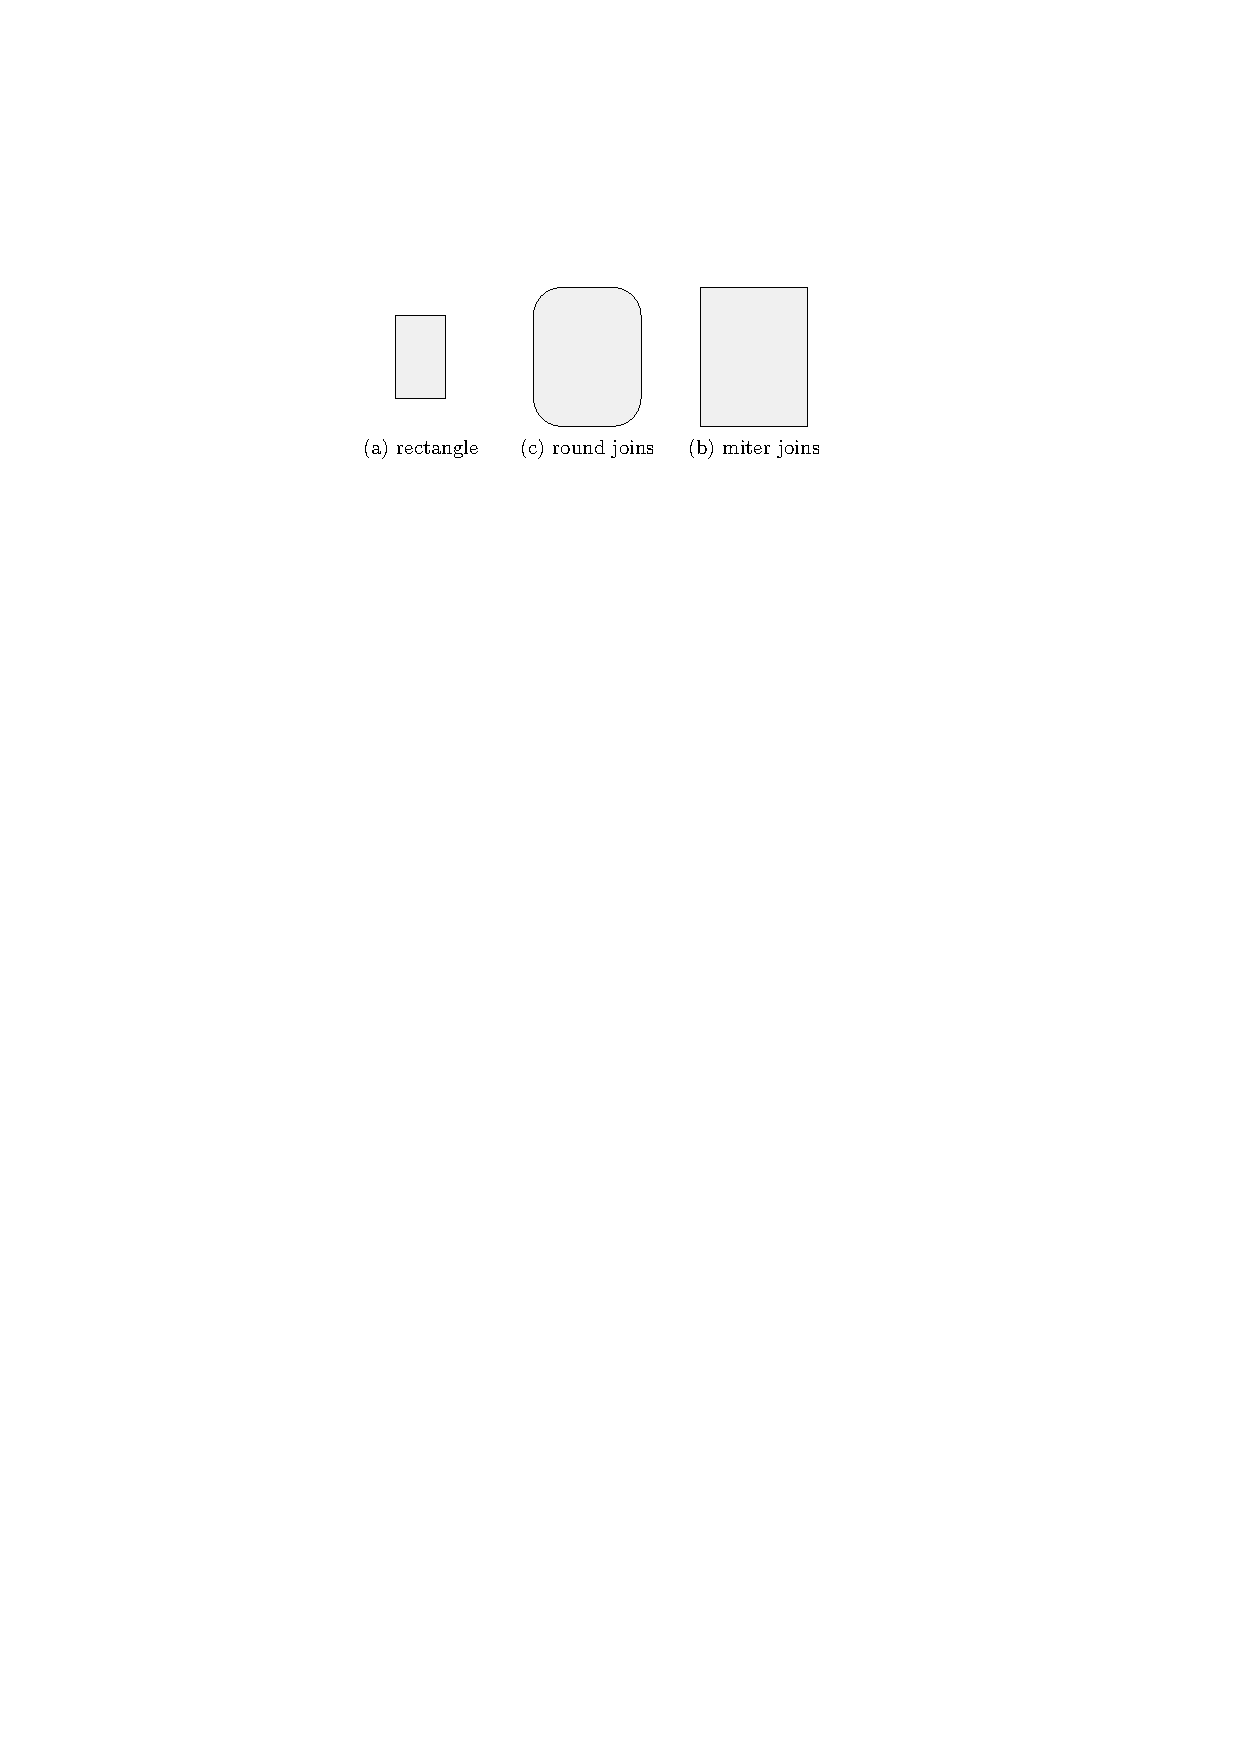
\includegraphics{Buffer_TwoKinds}
	\caption{Buffering a polygon using round joins and using miter joins.}
	\label{fig:Buffer_TwoKinds}
\end{figure}

\begin{figure}[tb]
	\centering
	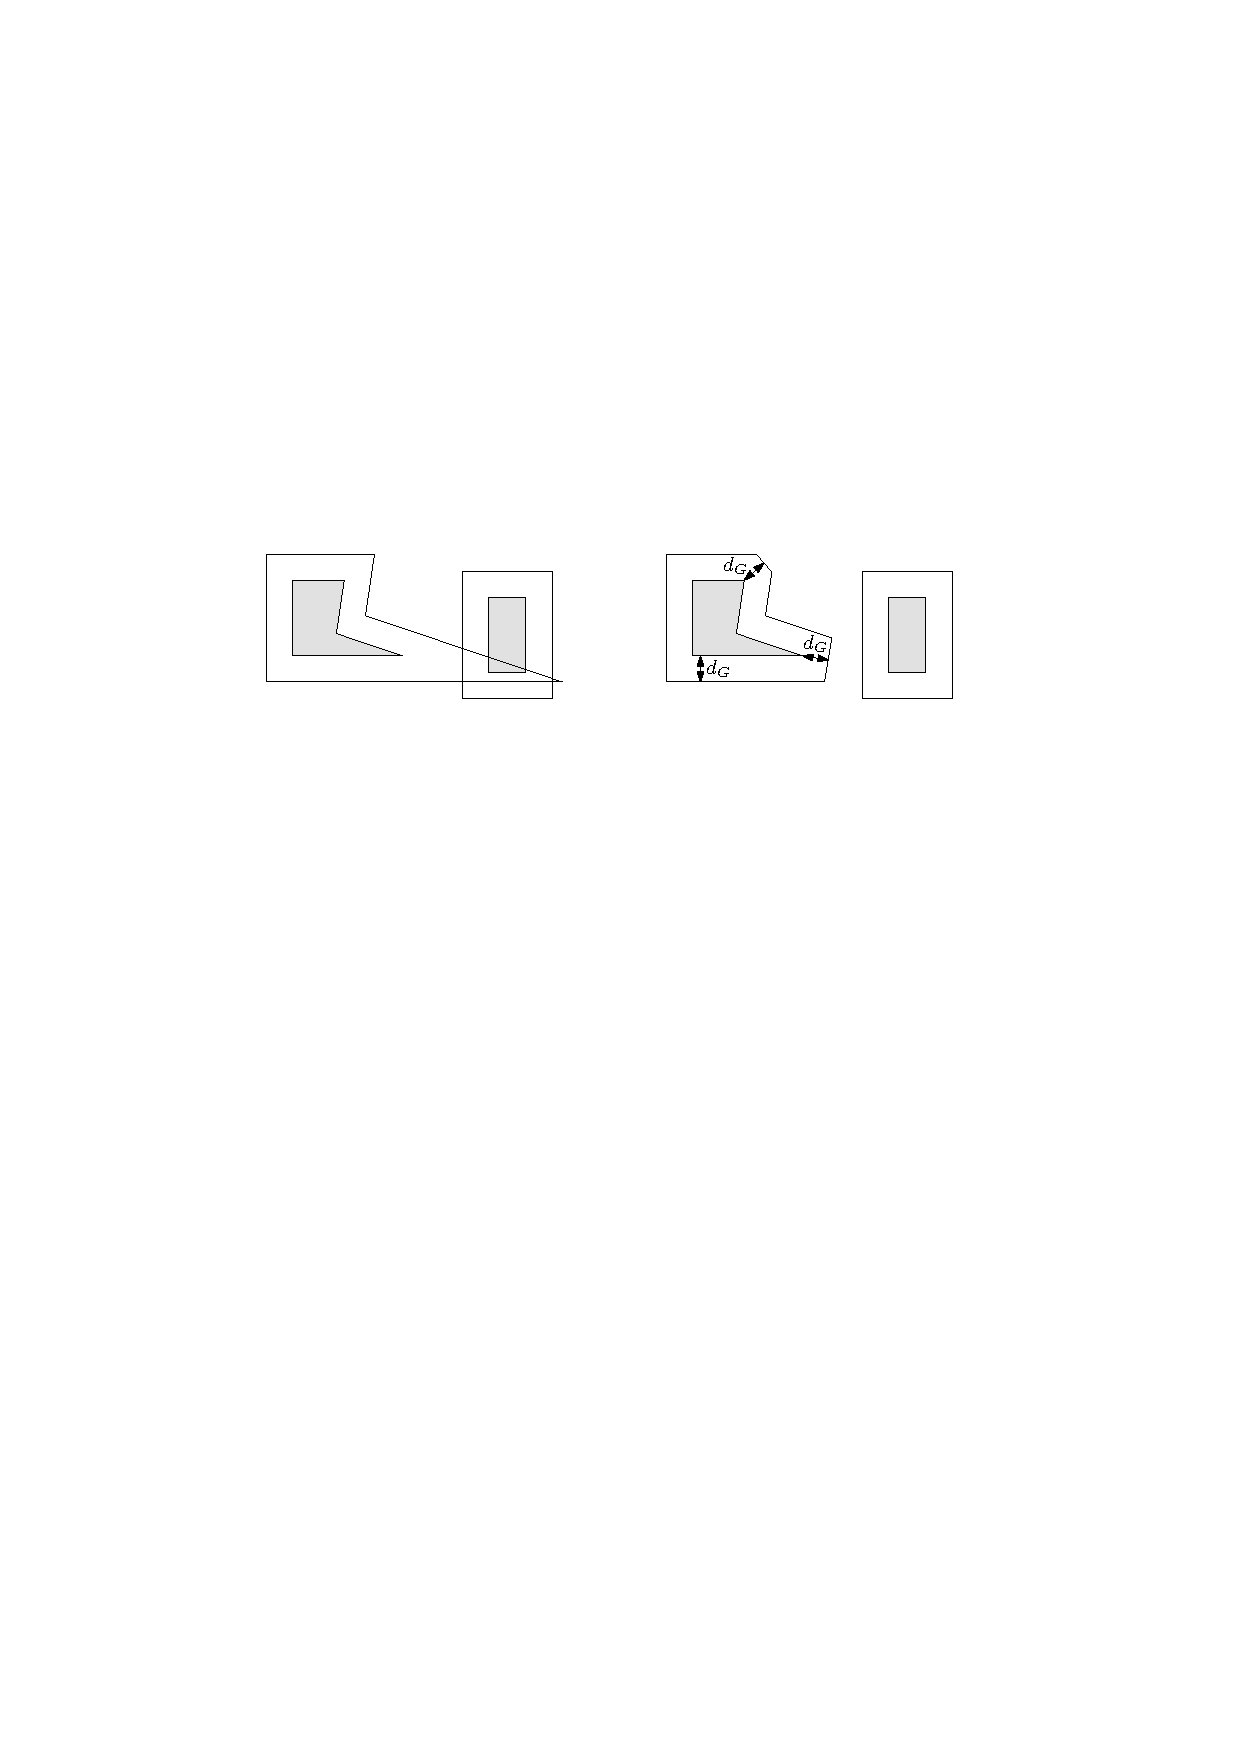
\includegraphics{Buffer_MiterLimits}
	\caption{Using square joins instead of miter joins to avoid long spikes.
	}
	\label{fig:Buffer_MiterLimits}
\end{figure}




\subsection{Simplifying grown buildings based on dilation and erosion}
\label{sec:DilationErosion}
As mentioned earlier, building simplification methods have already been 
proposed. \citet{Damen2008} generalized buildings using morphological operators.
A drawback of this method is that the orientation of the buildings have to be 
identified.
\citet{Meijers2016} simplified buildings 
based on offset curves generated from straight skeletons.
Our method is similar to \citet{Meijers2016}.
Our proposition is to dilate and erode the buildings, to remove dents and 
bumps that can occur when buildings grow.
(see \fig\ref{fig:RemoveDentAndBump}).
The operations of dilation and erosion are available from library 
\textsc{Clipper} \citep{Johnson2014}.

\begin{figure}[tb]
	\centering
	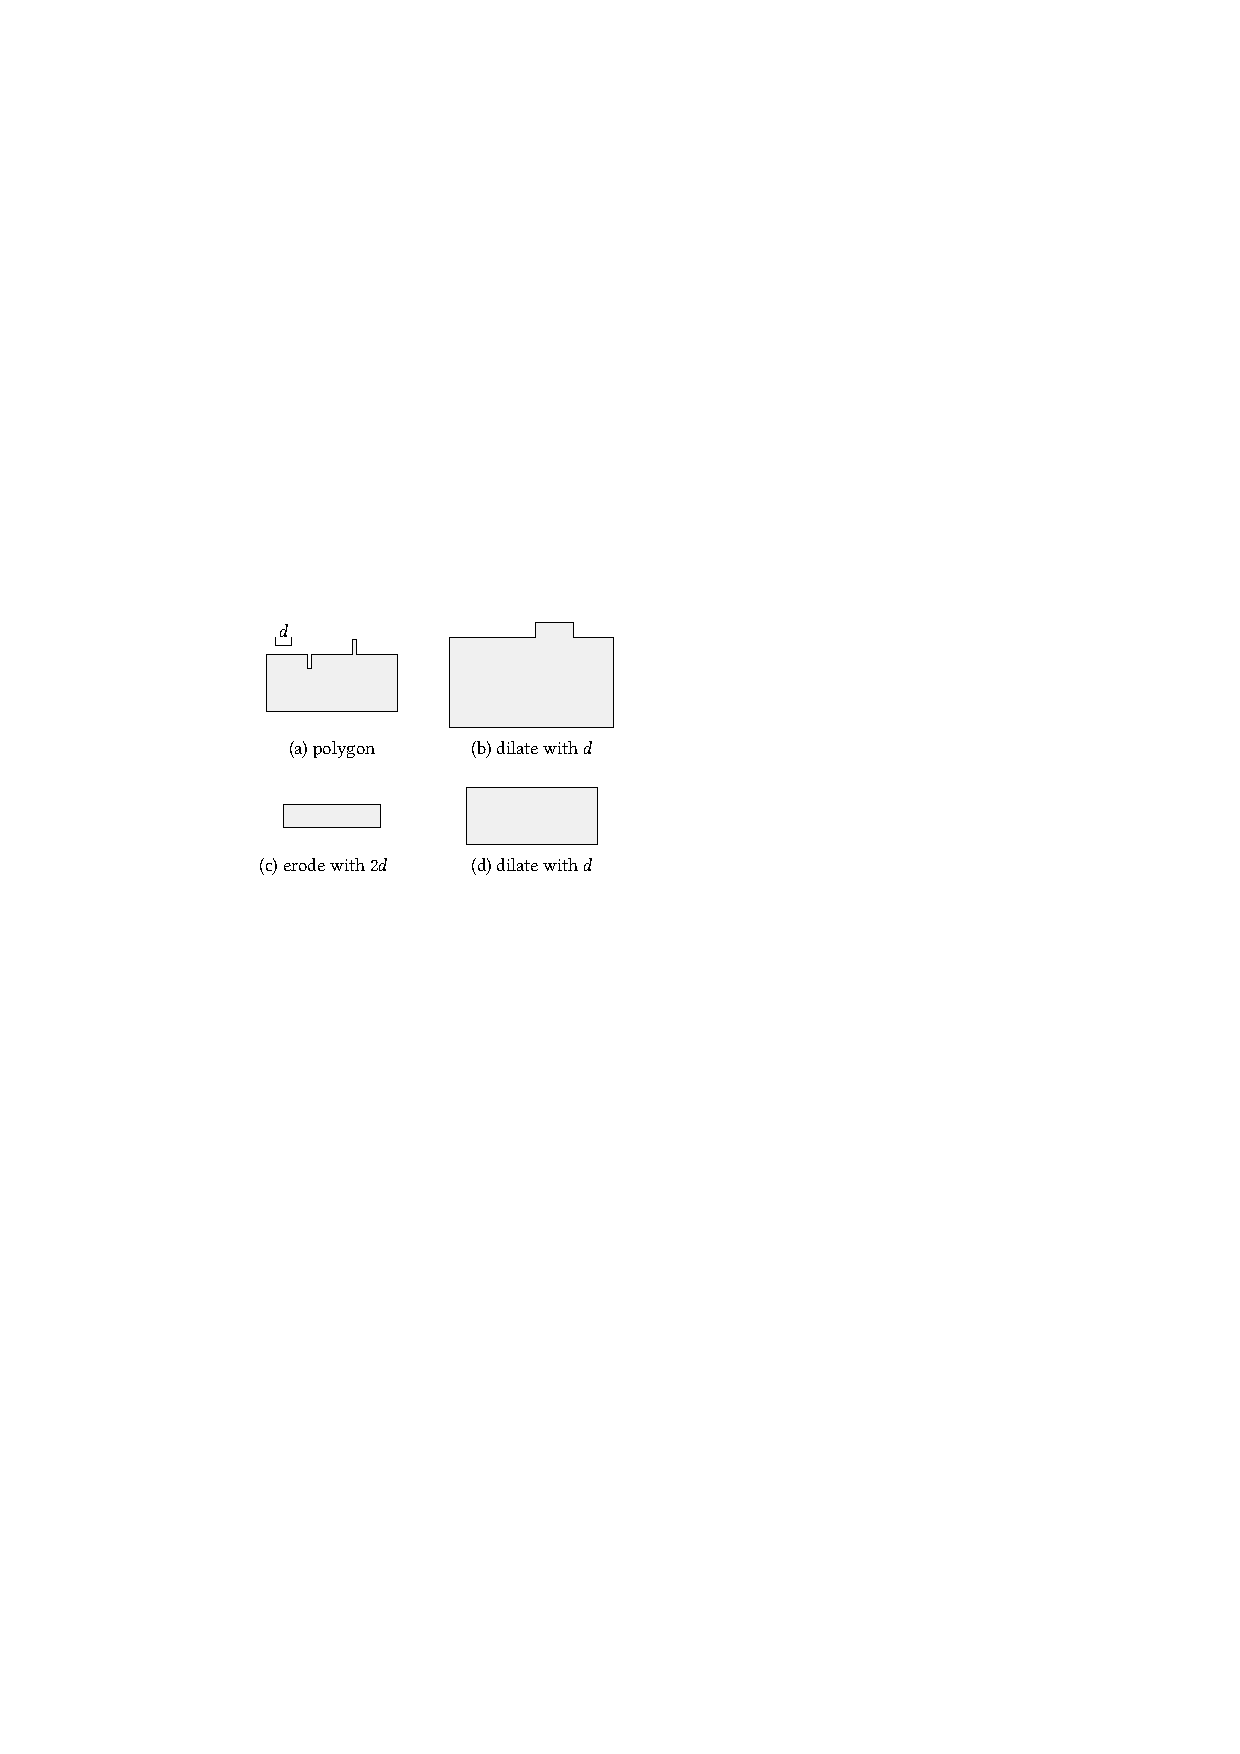
\includegraphics[]{RemoveDentAndBump}
	\caption{Removing a dent by dilating and then remove a bump by eroding.
		(a) a polygon with a dent and a bump;
		(b) dilating the polygon in (a) with distance $d$ to remove the dent;
		(c) eroding the polygon in (b) with $2d$ to remove the bump;
		(d) dilating the polygon in (c) with $d$ so that the result has 
		the same size as the polygon in (a).
	}
	\label{fig:RemoveDentAndBump}
\end{figure}

At time $t$, we grow buildings with distance $\dtrm{G}$.
We dilate with distance $\dtrm{D}$ ($\dtrm{D}>0$),
erode with $\dtrm{D}+\dtrm{E} (\dtrm{E}>0)$,
and dilate back with $\dtrm{E}$.
A problem we may have is that 
a building may be split into several parts by erosion
(see \fig\ref{fig:ErosionBreak} for example).
The reason is that 
some parts of a building may be increased (by growing and dilating) 
with distance $\dtrm{G}+\dtrm{D}$, 
but can be decreased (by eroding) as much as $\alpha (\dtrm{D}+\dtrm{E})$.
If $\dtrm{G}+\dtrm{D} < \alpha (\dtrm{D}+\dtrm{E})$ 
and the building is not thick enough, 
a thin part may disappear.
In order to avoid this problem, we require that
\[
\dtrm{G} + \dtrm{D} \ge \alpha (\dtrm{D}+\dtrm{E}),
\]
which means
\begin{equation}
\label{eq:d_Dt}
\dtrm{D} \le \frac{\dtrm{G}-\dtrm{E}}{\alpha - 1}.
\end{equation}

\begin{figure}[tb]
	\centering
	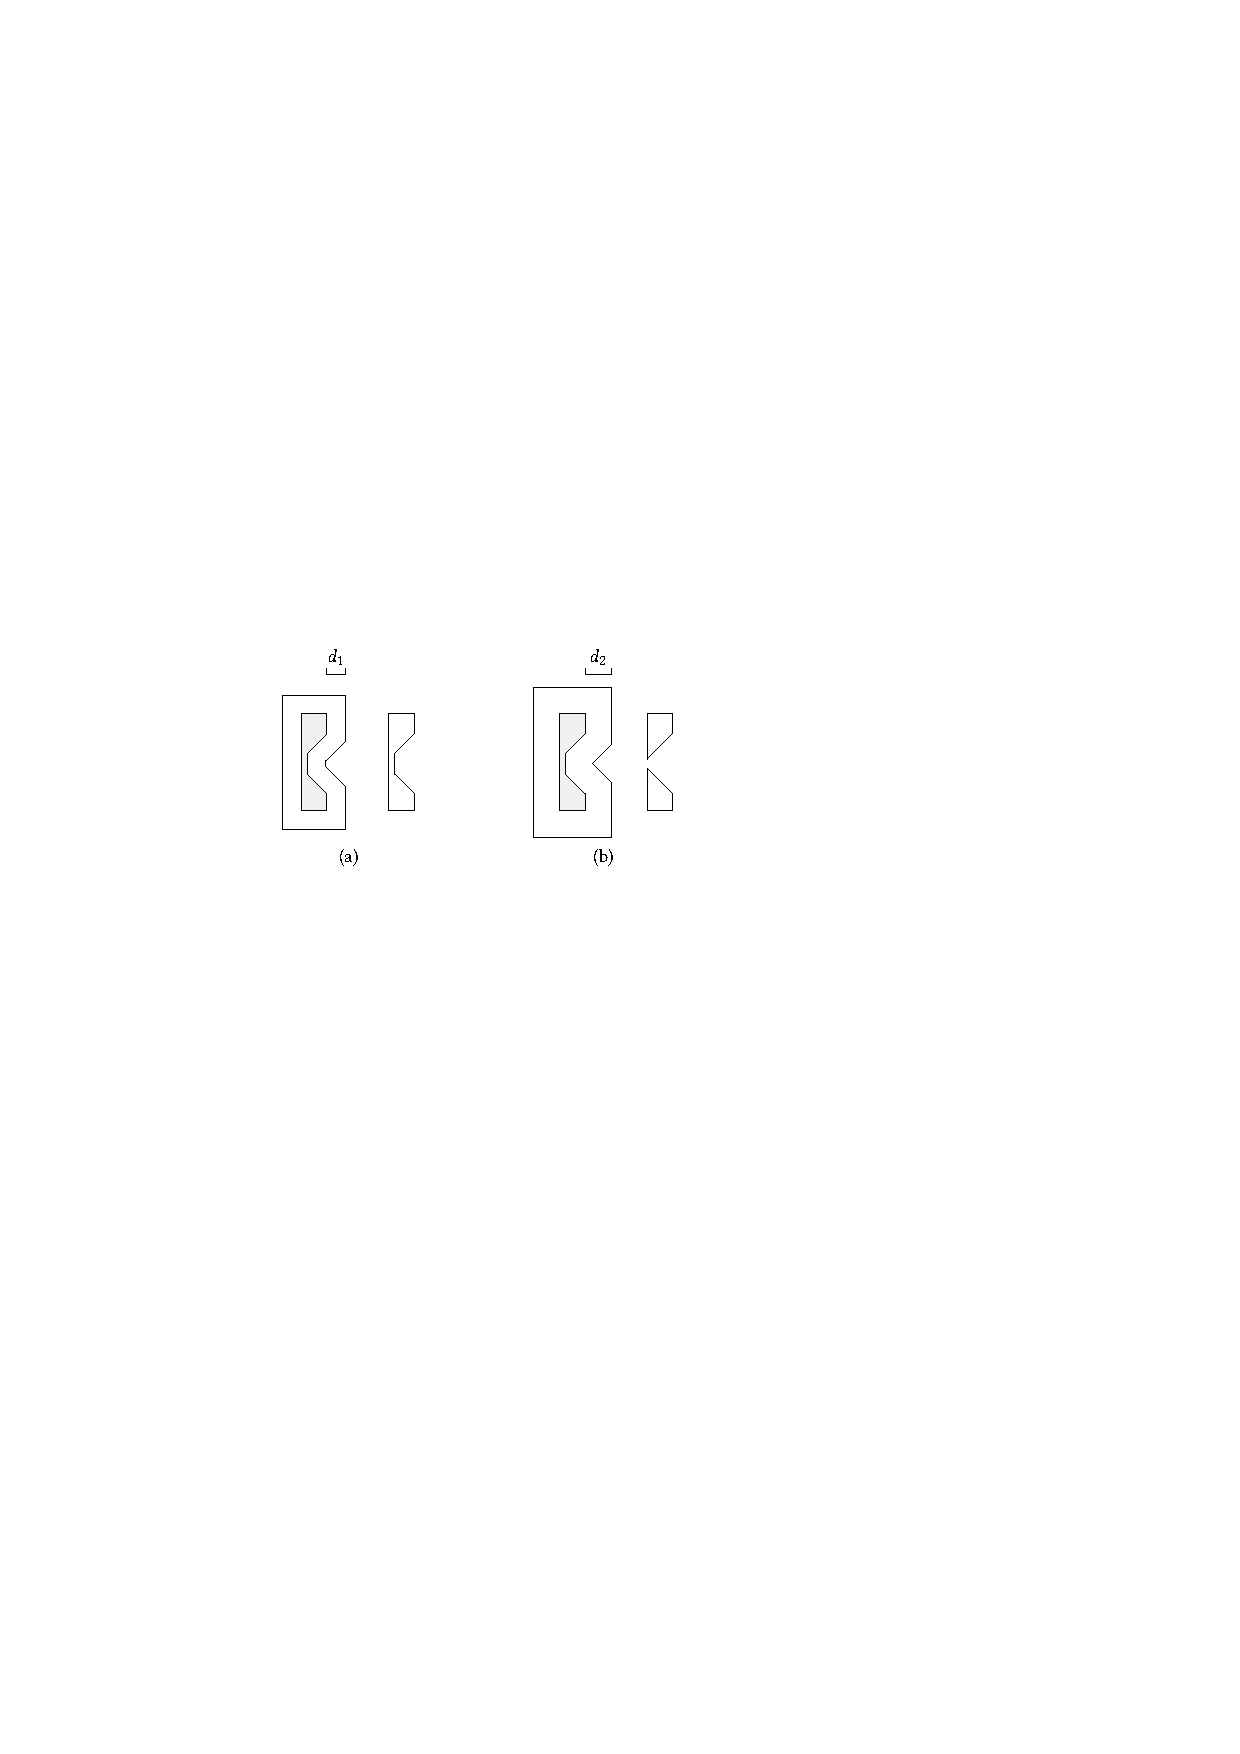
\includegraphics[]{ErosionBreak}
	\caption{Dilating the gray polygon, then eroding the dilated polygon.
		(a) Dilating and eroding with distance $d_1$.
		(b) Dilating and eroding with $d_2$, where $d_2>d_1$.
		In (a) the result of dilation and erosion is the same as the original 
		polygon, while in (b) the result consists of two parts.
	}
	\label{fig:ErosionBreak}
\end{figure}

We would like to use $\dtrm{E}=\frac{l}{2} \cdot M_t$ so that
any dents and bumps narrower than $l$ will be removed. 
We set $l=0.3\,\mathrm{mm}$ in the map, 
which was used as a length threshold by, for example, 
\citet{Regnauld2001}.
Unfortunately, distance $\dtrm{G}$ can be arbitrarily small 
according to \eq\ref{eq:d_Gt}, 
but $\dtrm{E}$ is at least $\frac{l}{2} M_\mathrm{s}$. 
In this case, $\dtrm{G}-\dtrm{E} \le 0$ when $t$ is small, 
which violates \eq\ref{eq:d_Dt}, where $\dtrm{D}>0$.
As a compromise, we set erosion distance
\begin{equation}
\label{eq:d_Et}
\dtrm{E} =t \cdot \frac{l}{2} M_\mathrm{g}.
\end{equation}
%Still, we should make sure that $\dtrm{G}-\dtrm{E} > 0$, which means
%$t \cdot \frac{\lambda}{2}\sqrt{a} (M_\mathrm{g}-M_\mathrm{s})-
%t \cdot \frac{l}{2} M_\mathrm{g} >0$.
Still, we have to make sure that $\dtrm{G}-\dtrm{E} > 0$, which means
$t \cdot d_\mathrm{G} - t \cdot \frac{l}{2} M_\mathrm{g} >0$.
As a result, we need to make sure that
\begin{equation}
\label{eq:S_g}
M_\mathrm{g} < \frac{2 d_\mathrm{G}}{l}.
\end{equation}

We wish to remove ``bays'' 
which have ``widths'' less than $2 r_\mathrm{h}$. 
Variable $r_\mathrm{h}= 2\sqrt{a_\mathrm{h}/\pi}$
is the radius of a hole which is just large enough to be presented on map.
Following \citep{Chaudhry2008}, we set area $a_\mathrm{h} = 8\,\mathrm{mm}^2$ 
in the map.
Sometimes, our $\dtrm{D}$ is not large enough to do so 
because of the limitation from \eq\ref{eq:d_Dt}.
We define
\[
\dtrm{D} =\min (\frac{\dtrm{G}-\dtrm{E}}{\alpha - 1}, r_\mathrm{h} M_t) .
\]

\todo{please explain in a figure what a bay is, and what is the width of the 
bay}

\subsection{Iteratively aggregating close buildings by adding bridges}
\label{sec:Aggregate}


We grow each original building and, as illustrated in 
\sect\ref{sec:DilationErosion}, simplify the grown building.
If some buildings become too close after these operations,
we aggregate them by adding bridges
(see for example \fig\ref{fig:GrowAndBridge}).
Following \citet{Stoter2009}, 
we define that two buildings are too close if their distance is less than
$\epsilon= 0.2\,\mathrm{mm}$ on map.
The real separation threshold at time $t$ is
\begin{equation}
\label{eq:d_epsilont}
d_{\epsilon, t} = \epsilon \cdot M_t.
\end{equation}

\begin{figure*}[tb]
	\centering
	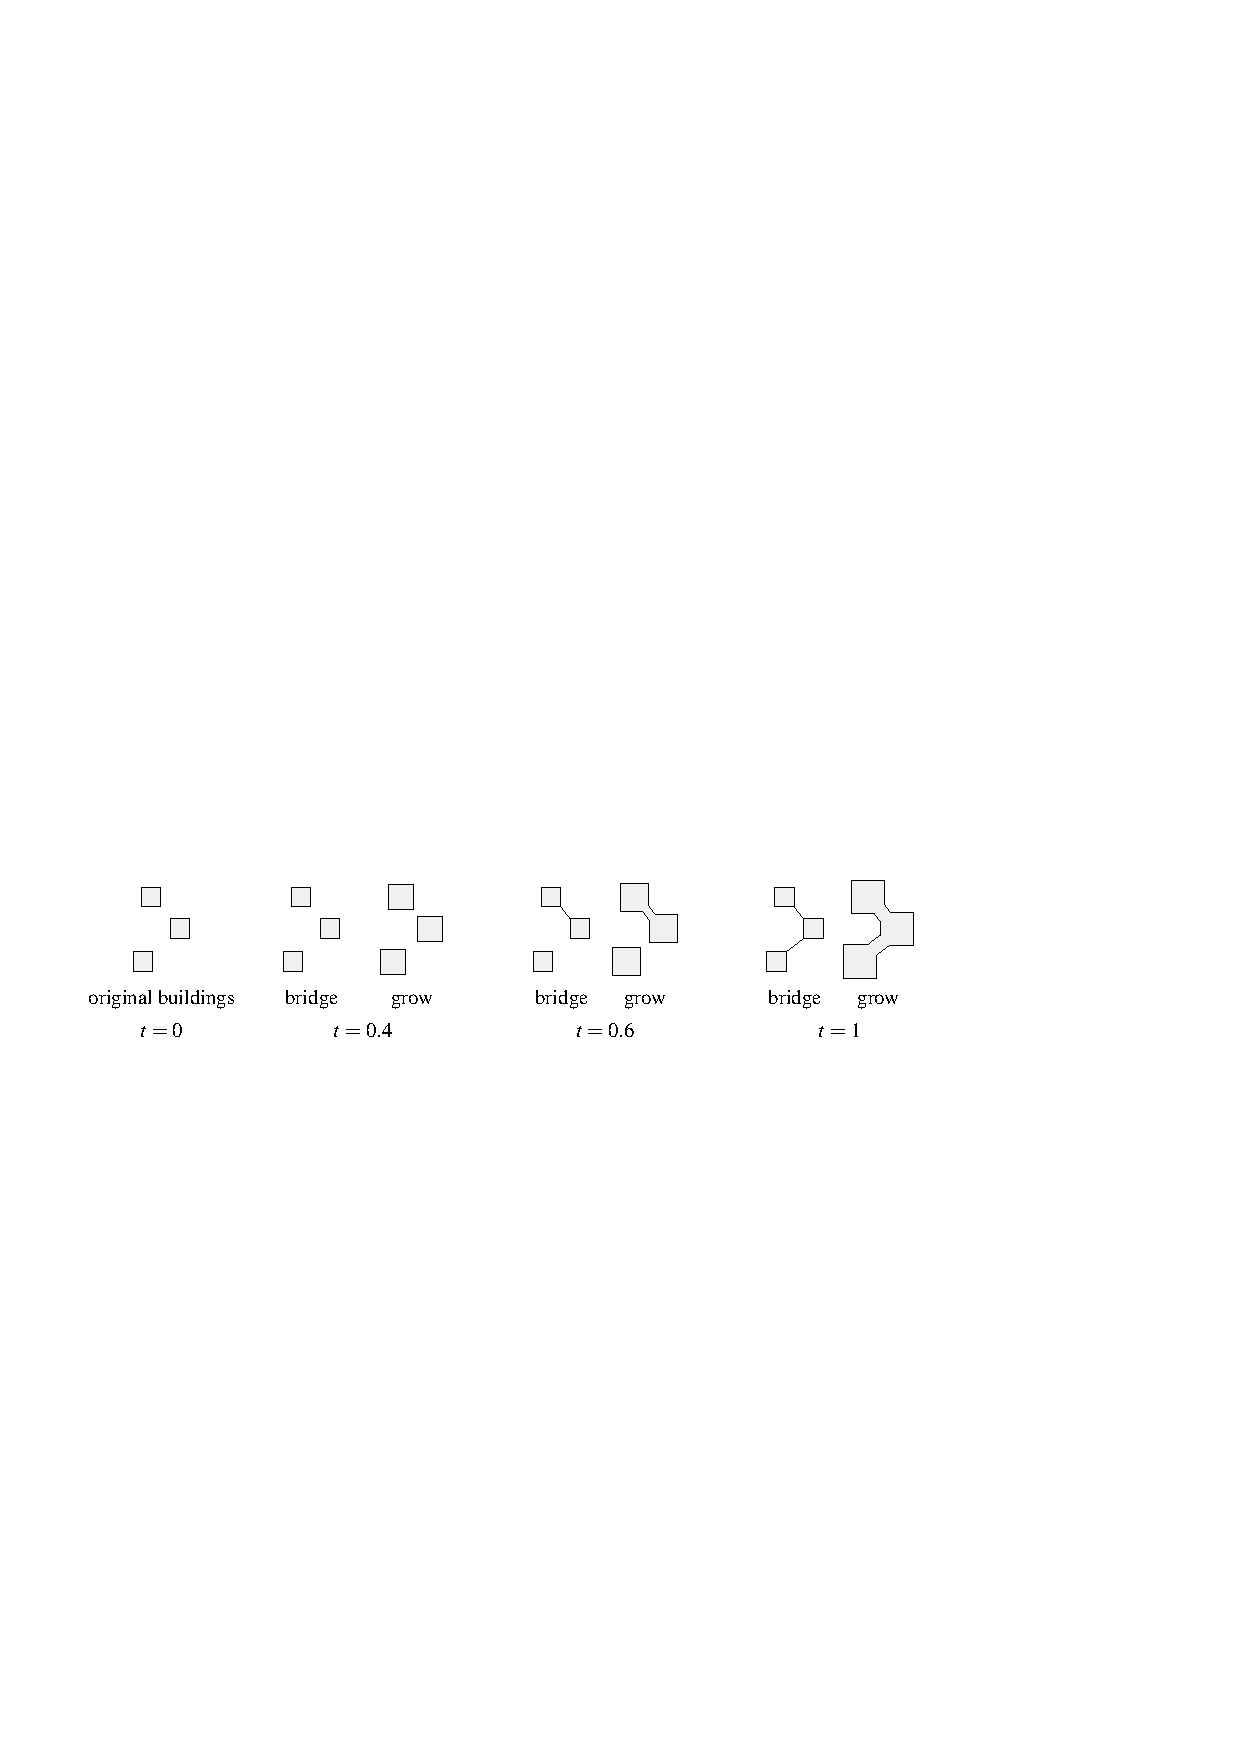
\includegraphics[draft=false]{GrowAndBridge}
	\caption{Aggregating original buildings in the same group by introducing 
		bridges.
		Then grow the bridged buildings.}
	\label{fig:GrowAndBridge}
\end{figure*}

Our way of detecting close buildings is simple.
We buffer buildings with distance $d_{\epsilon, t}/2$ using round joins.
We merge the buffers that overlap each other.
The buildings intersect the same merged buffer 
are identified as a group of close buildings.
The corresponding original buildings 
are identified as a group of original close buildings.
For each pair of the original buildings in the same group,
we connect them by adding a line segment linking the nearest points.
The line segments for a group of original buildings may cross each other or 
even intersect buildings.
To make the topology simple, 
we only select some of the line segments as \emph{bridges}.  
We consider each building as a node and each line segment as an edge, 
then we have a graph.
Using Prim's algorithm \citep{Prim1957}, 
we find a minimum spanning tree (MST) in the graph,
taking the lengths of the line segments as the weights.
As a results, the line segments corresponding to the edges in the MST
are identified as bridges.
We aggregate the group of original buildings by adding these bridges.

Aggregated buildings may become too close because of the additional bridges.
Therefore we have to iterate the aggregation process.
\fig\ref{fig:BridgeMoreBuilding} shows such an example.
For example, we grow and buffer buildings $p$, $q$, and~$r$.
As the buffers of $q$ and~$r$ overlap
(see \fig\ref{fig:BridgeMoreBuilding}c),
we aggregate buildings $q$ and~$r$ by adding a bridge
(see \fig\ref{fig:BridgeMoreBuilding}d).
There are two buildings left in \fig\ref{fig:BridgeMoreBuilding}d.
We then grow and buffer the buildings in 
\fig\ref{fig:BridgeMoreBuilding}d, 
the buffer of building $p$ overlap the buffer of the bridge for $q$ and $r$
(see \fig\ref{fig:BridgeMoreBuilding}f).
Finally, building $p$ is aggregated with bridged $q$ and $r$
(see \fig\ref{fig:BridgeMoreBuilding}g), and
there is only one building left in \fig\ref{fig:BridgeMoreBuilding}g.
Then we grow and buffer again to get the final geometry of the group.
As the number of buildings does not decrease comparing to last process (one 
building before, one building after),
the iteration stops.

\begin{figure}[tb]
	\centering
	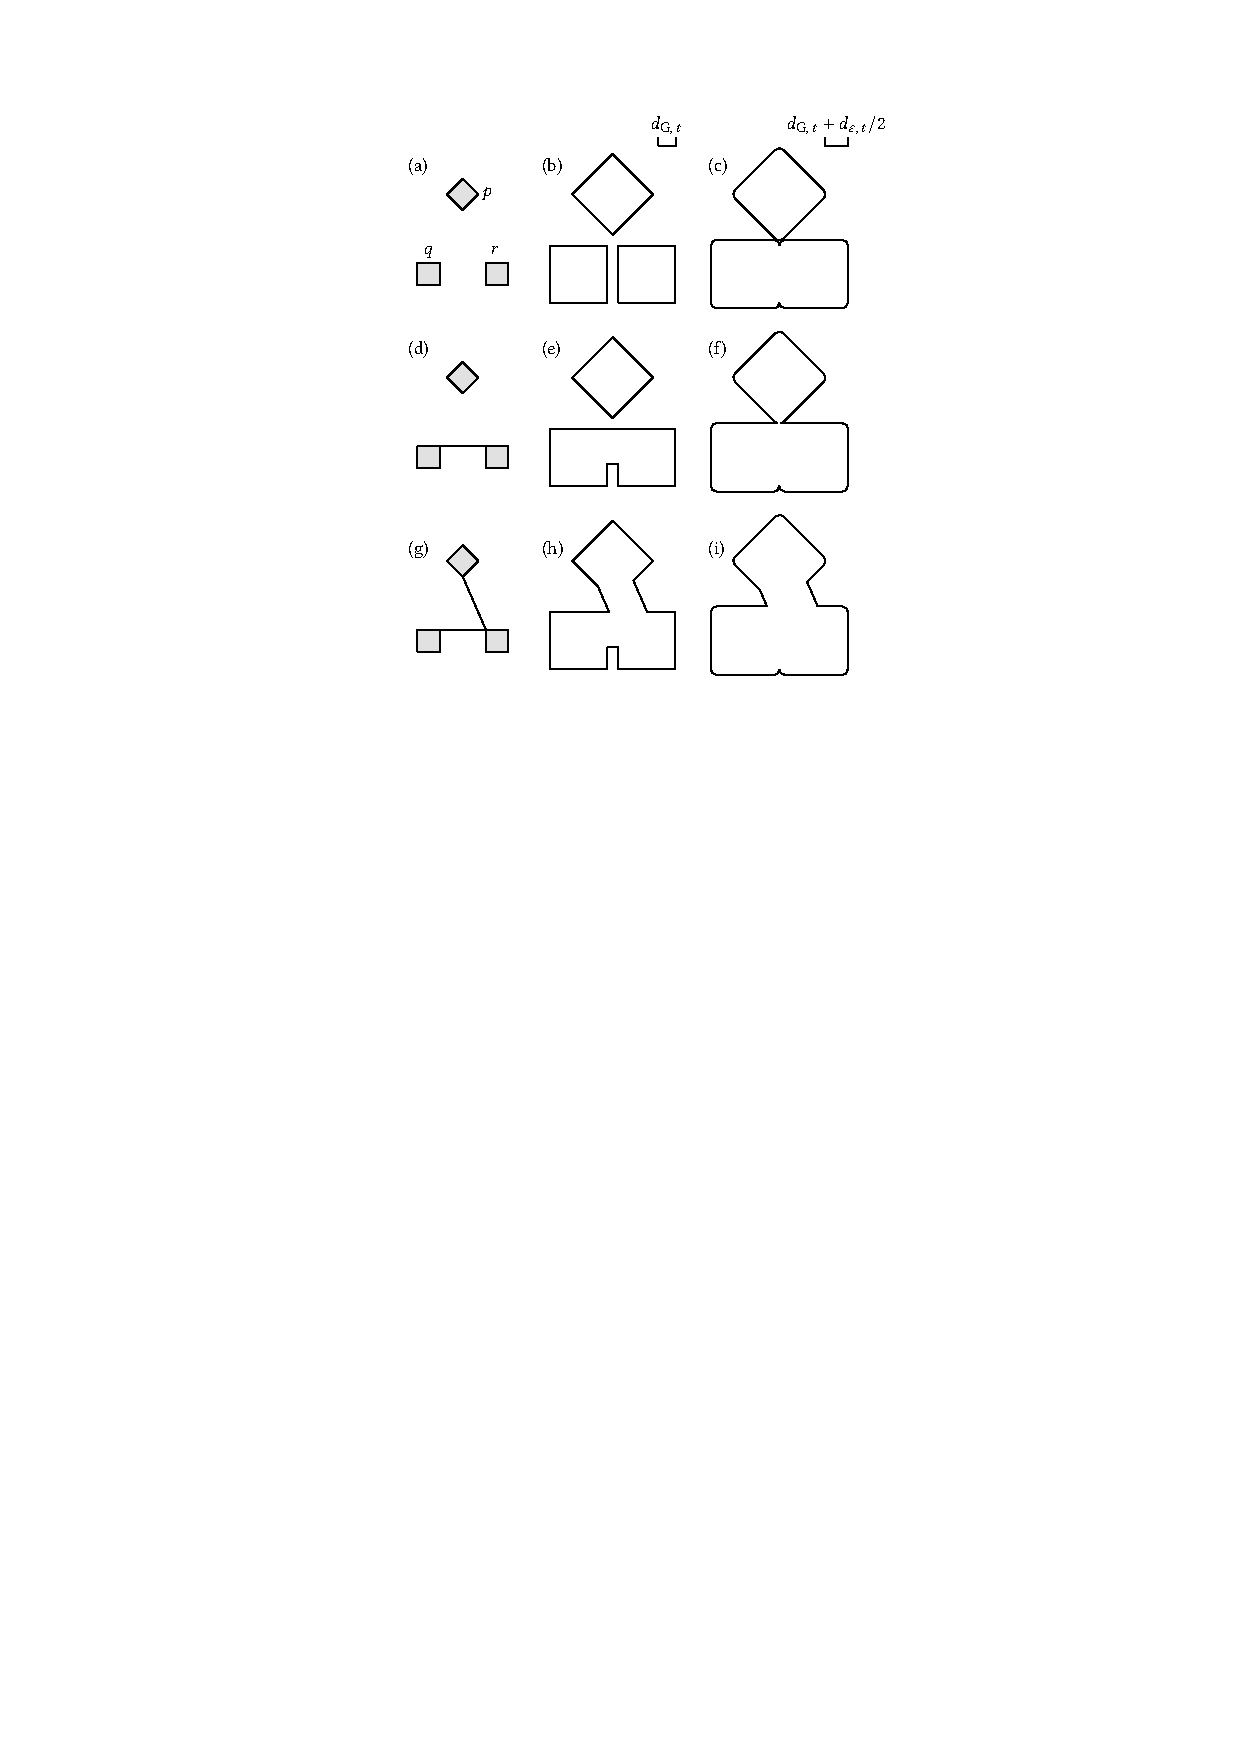
\includegraphics[draft=false]{BridgeMoreBuilding}
	\caption{Iteratively aggregating close buildings by adding bridges.
		(a) original buildings $p$, $q$, and~$r$.
		(b) growing the original buildings with distance $\dtrm{G}$.
		(c) buffering the grown buildings with distance $d_{\epsilon,t}/2$ 
		using round joins.
		(d) aggregating buildings $q$ and~$r$ by adding a bridge,
		as their buffer overlap each other in (c).
		(e) growing the buildings in (d) with distance $\dtrm{G}$.
		(f) buffering the grown buildings in (e) with distance 
		$d_{\epsilon,t}/2$ using round joins.
		(g) aggregating buildings $p$, $q$ and~$r$ by adding bridges.
		(h) growing the buildings in (g) with distance $\dtrm{G}$.
		(i) buffering the grown buildings in (h) with distance 
		$d_{\epsilon,t}/2$ using round joins.
	}
	\label{fig:BridgeMoreBuilding}
\end{figure}


%At any time $t$, some of the bridges are picked to aggregate buildings 
%which grow to become too close.
%The buildings and the bridges already comprise some MSTs.



%
%Original buildings grow according to time $t$.
%We put the original buildings in the same group if 
%they grow so that their distance is less than $d_{\epsilon, t}$.
%Following \citet{Stoter2009}, 
%we set the threshold $\epsilon= 0.2\,\mathrm{mm}$ on map. 
%The real separation threshold at time $t$ is
%\begin{equation}
%\label{eq:d_epsilont2}
%d_{\epsilon, t} = \epsilon \cdot M_t.
%\end{equation}
%We group buildings based on buffering.
%The basic idea is that 
%we buffer the original buildings with distance $\dtrm{G}$
%and an additional distance $d_{\epsilon, t}/2$
%(the distance between two buildings should be at least $d_{\epsilon, t}$).
%If two buffers overlap, 
%then the original buildings are put in the same group.
%However, as some parts of a building grow faster than other parts, 
%this basic idea may cause problems.
%An example is shown in \fig\ref{fig:CloseDetect}c and~d.
%In \fig\ref{fig:CloseDetect}d, 
%the buffers of buildings $p$ and $q$ overlap each other.
%So we should aggregate buildings $p$ and $q$ at time $t$
%because they will grow to become too close.
%According to the bridges in \fig\ref{fig:CloseDetect}b, 
%buildings $p$ and $q$ should be aggregated via building $r$.
%Unfortunately, neither $p$ or $q$ will be too close to $r$.
%As we use bridges to aggregate buildings 
%(see \sect\ref{sec:Aggregate}),
%we are not able to aggregate buildings $p$ and $q$. 
%To avoid this situation, 
%we buffer original buildings with distance
%$\alpha \dtrm{G}+d_{\epsilon, t}/2$ using round joins.
%This buffering guarantees 
%that every part of a building grows with the same speed.
%If the buffers of two buildings overlap each other,
%then the two buildings are surely aggregated into one.
%Using this buffering, in most of cases 
%two buildings are aggregated as soon as 
%their separation distance is less than 
%$2(\alpha -1) \dtrm{G}+d_{\epsilon, t}$.
%The advantage is that we guarantee that 
%any two buildings have separate distance less than $d_{\epsilon, t}$ will be 
%aggregated via bridges.
%
%\begin{figure}[tb]
%	\centering
%	
\includegraphics[]{NearestPoints}
%	\caption{The nearest points between a pair of buildings may change because 
%		of growing. 
%		The two squares and the two circles respectively mark
%		the nearest points before and after growing.
%	}
%	\label{fig:NearestPoints}
%\end{figure}


\subsection{Simplifying aggregated buildings using Imai--Iri algorithm}
\label{sec:ImaiIri}

When buildings are grown and aggregated iteratively, bridges are added, 
and these bridges have a width of $2\dtrm{G}$ at time $t$.
This setting guarantees that no bridge is thin when $t=1$.

This agrregation process creates new small details that need to be removed. So, 
the aggregated buildings are simplified using Imai--Iri algorithm 
\citep{ImaiIri1988}.
First, this algorithm finds all the valid shortcuts of a polyline.
A shortcut is valid for a segment 
if the distance between the segment and the shortcut is at most a specified 
value
(see \fig\ref{fig:ImaiIri_Shortcut}).
We set the value also as $l$.
That is, at time $t$, the threshold distance is
\begin{equation}
\label{eq:d_lt}
d_{l,t}= l \cdot M_t.
\end{equation}
Second, the algorithm finds a sequence of valid shortcuts, from the beginning 
of a polyline to the end, using breadth-first search.
The sequence of valid shortcuts is an approximation of the polyline 
and has the least number of line segments, with error smaller than $d_{l,t}$.

\begin{figure}[tb]
	\centering
	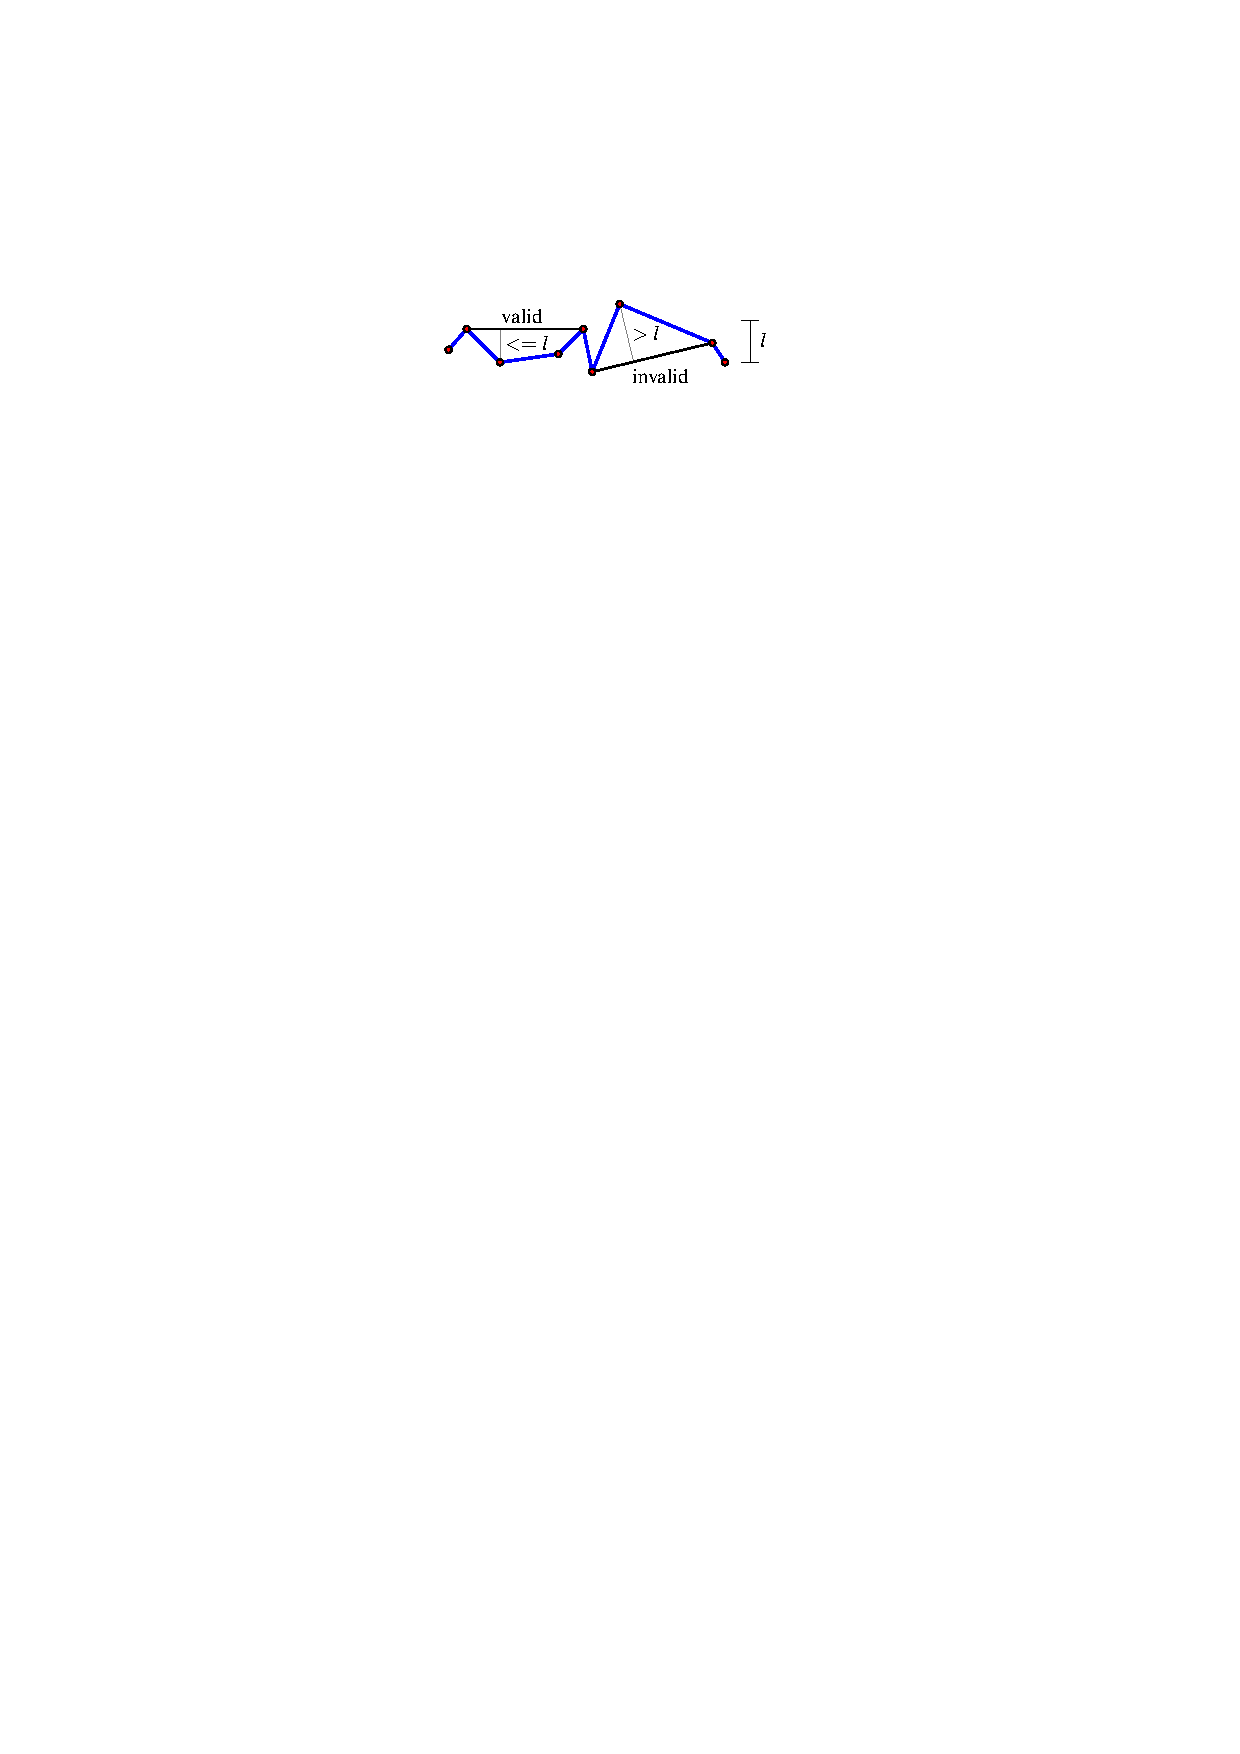
\includegraphics[]{ImaiIri_Shortcut}
	\caption{Valid and invalid shortcuts for Imai--Iri algorithm.}
	\label{fig:ImaiIri_Shortcut}
\end{figure}

We add two more constraints for a shortcut to be valid. 
First, a shortcut must be completely inside the grown building.
If a shortcut is outside,
we are not able to arrive at the shortcut by growing.
Second, a shortcut is not allowed to intersect the aggregated building.
If we allow this intersection, 
the building will have to be shrunk, which should be avoided. 


The classical way to filter points in a polyline or polygon is the 
Douglas--Peucker algorithm \citep{Douglas1973}, 
but it did not filter enough the geometry, or damaged too much the shapes when 
the threshold was bigger, so the Imai--Iri 
algorithm was chosen as a better fit. 

%\subsection{Grouping buildings based on buffering}
%\label{sec:Group}
%There are many research works about grouping buildings.
%\citet{Cetinkaya2015} and \citet{Deng2017} compared some of the methods.
%However, our two needs, 
%the distances between buildings are always larger than a specified threshold 
%and small bays should be removed, 
%motivate us to develop our own grouping method.
%
%Original buildings grow according to time $t$.
%We put the original buildings in the same group if 
%they grow so that their distance is less than $d_{\epsilon, t}$.
%Following \citet{Stoter2009}, 
%we set the threshold $\epsilon= 0.2\,\mathrm{mm}$ on map. 
%The real separation threshold at time $t$ is
%%\begin{equation}
%%\label{eq:d_epsilont}
%%d_{\epsilon, t} = \epsilon \cdot M_t.
%%\end{equation}
%We group buildings based on buffering.
%The basic idea is that 
%we buffer the original buildings with distance $\dtrm{G}$
%and an additional distance $d_{\epsilon, t}/2$
%(the distance between two buildings should be at least $d_{\epsilon, t}$).
%If two buffers overlap, 
%then the original buildings are put in the same group.
%However, as some parts of a building grow faster than other parts, 
%this basic idea may cause problems.
%An example is shown in \fig\ref{fig:CloseDetect}c and~d.
%In \fig\ref{fig:CloseDetect}d, 
%the buffers of buildings $p$ and $q$ overlap each other.
%So we should aggregate buildings $p$ and $q$ at time $t$
%because they will grow to become too close.
%According to the bridges in \fig\ref{fig:CloseDetect}b, 
%buildings $p$ and $q$ should be aggregated via building $r$.
%Unfortunately, neither $p$ or $q$ will be too close to $r$.
%As we use bridges to aggregate buildings 
%(see \sect\ref{sec:Aggregate}),
%we are not able to aggregate buildings $p$ and $q$. 
%To avoid this situation, 
%we buffer original buildings with distance
%$\alpha \dtrm{G}+d_{\epsilon, t}/2$ using round joins.
%This buffering guarantees 
%that every part of a building grows with the same speed.
%If the buffers of two buildings overlap each other,
%then the two buildings are surely aggregated into one.
%Using this buffering, in most of cases 
%two buildings are aggregated as soon as 
%their separation distance is less than 
%$2(\alpha -1) \dtrm{G}+d_{\epsilon, t}$.
%The advantage is that we guarantee that 
%any two buildings have separate distance less than $d_{\epsilon, t}$ will be 
%aggregated via bridges.
%
%\begin{figure}[tb]
%	\centering
%	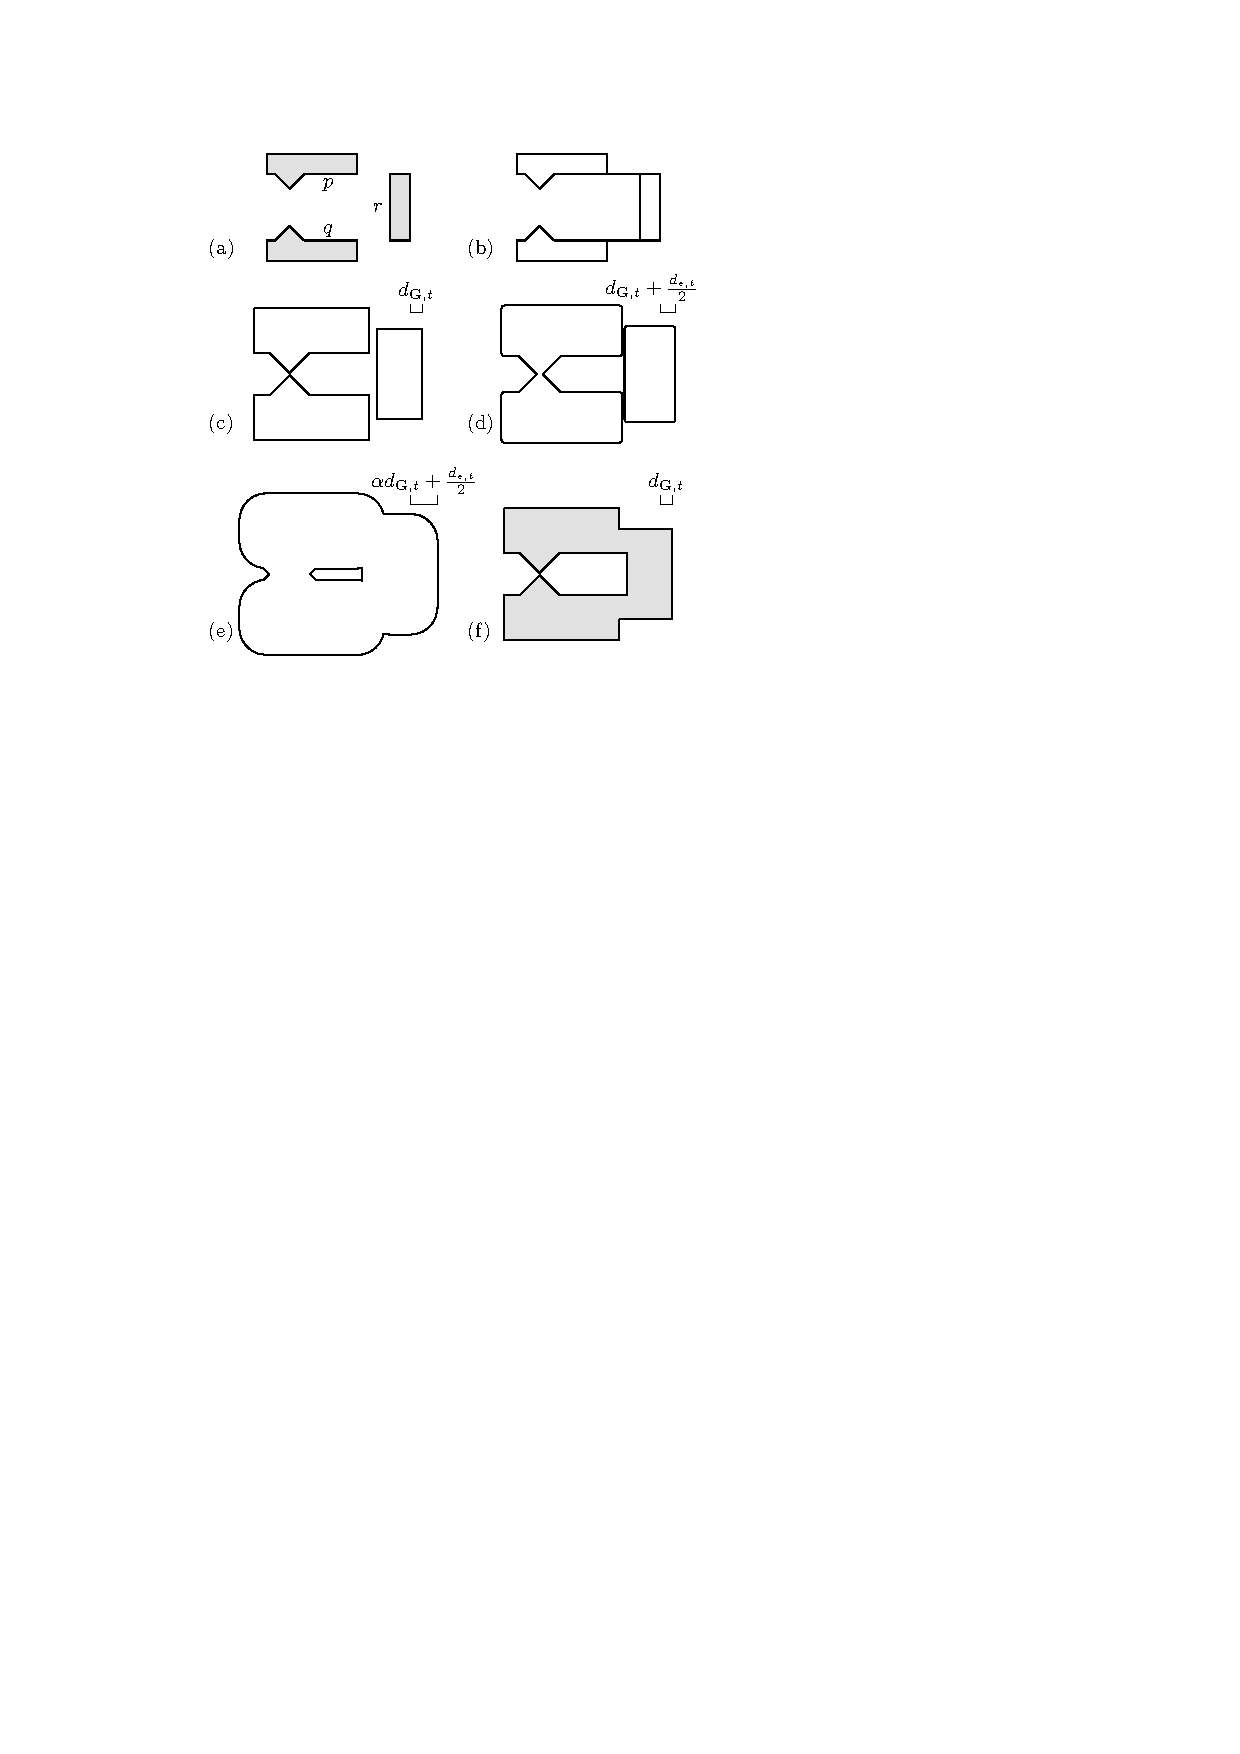
\includegraphics[]{CloseDetect}
%	\caption{Group buildings based on buffering.
%		(a) original buildings.
%		(b) bridges detected to aggregate the three buildings.
%		(c) grow the original buildings with distance $\dtrm{G}$.
%		(d) buffer the grown buildings in (c) 
%		with distance $d_{\epsilon, t} /2$ using round joins.
%		(e) buffer the original buildings 
%		with distance $\alpha \dtrm{G}+d_{\epsilon, t}/2 $ 
%		using round joins, where $\alpha=1.5$
%		(see \sect\ref{sec:Grow}).
%		(f) according to the buffer in (e), 
%		we put the three original buildings in the same group.
%		We aggregate the original buildings by adding the two bridges 
%		and grow the aggregated building with distance $\dtrm{G}$.
%	}
%	\label{fig:CloseDetect}
%\end{figure}


%
%As stated in \sect\ref{sec:DilationErosion}, 
%we wish to remove ``bays'' 
%which have widths less than $2 \dtrm{D}$.
%A bay may come from a complex original building,
%or from bridging some buildings.
%\fig\ref{fig:RemoveBay}e shows an example of the later case.
%To remove a bay,
%we overgrow (see \fig\ref{fig:RemoveBay}b and~e) 
%and then erode back (see \fig\ref{fig:RemoveBay}c and~f) 
%with distance $\dtrm{D}$.
%There may be some buildings in a bay (see \fig\ref{fig:RemoveBay}c),
%so we iteratively group until the number of groups does not decrease.
%For the buildings in \fig\ref{fig:RemoveBay}a,
%the final result of removing a bay is the outer polygon of 
%\fig\ref{fig:RemoveBay}h. 
%In comparison, the result is \fig\ref{fig:RemoveBay}e 
%if we do not dilate (setting $\dtrm{D}=0$) to remove a bay.
%Note that the pit we want to remove in \fig\ref{fig:RemovePitAndSpike} is a 
%kind of bay and will be removed by overgrowing.
%
%
%\begin{figure*}[tb]
%	\centering
%	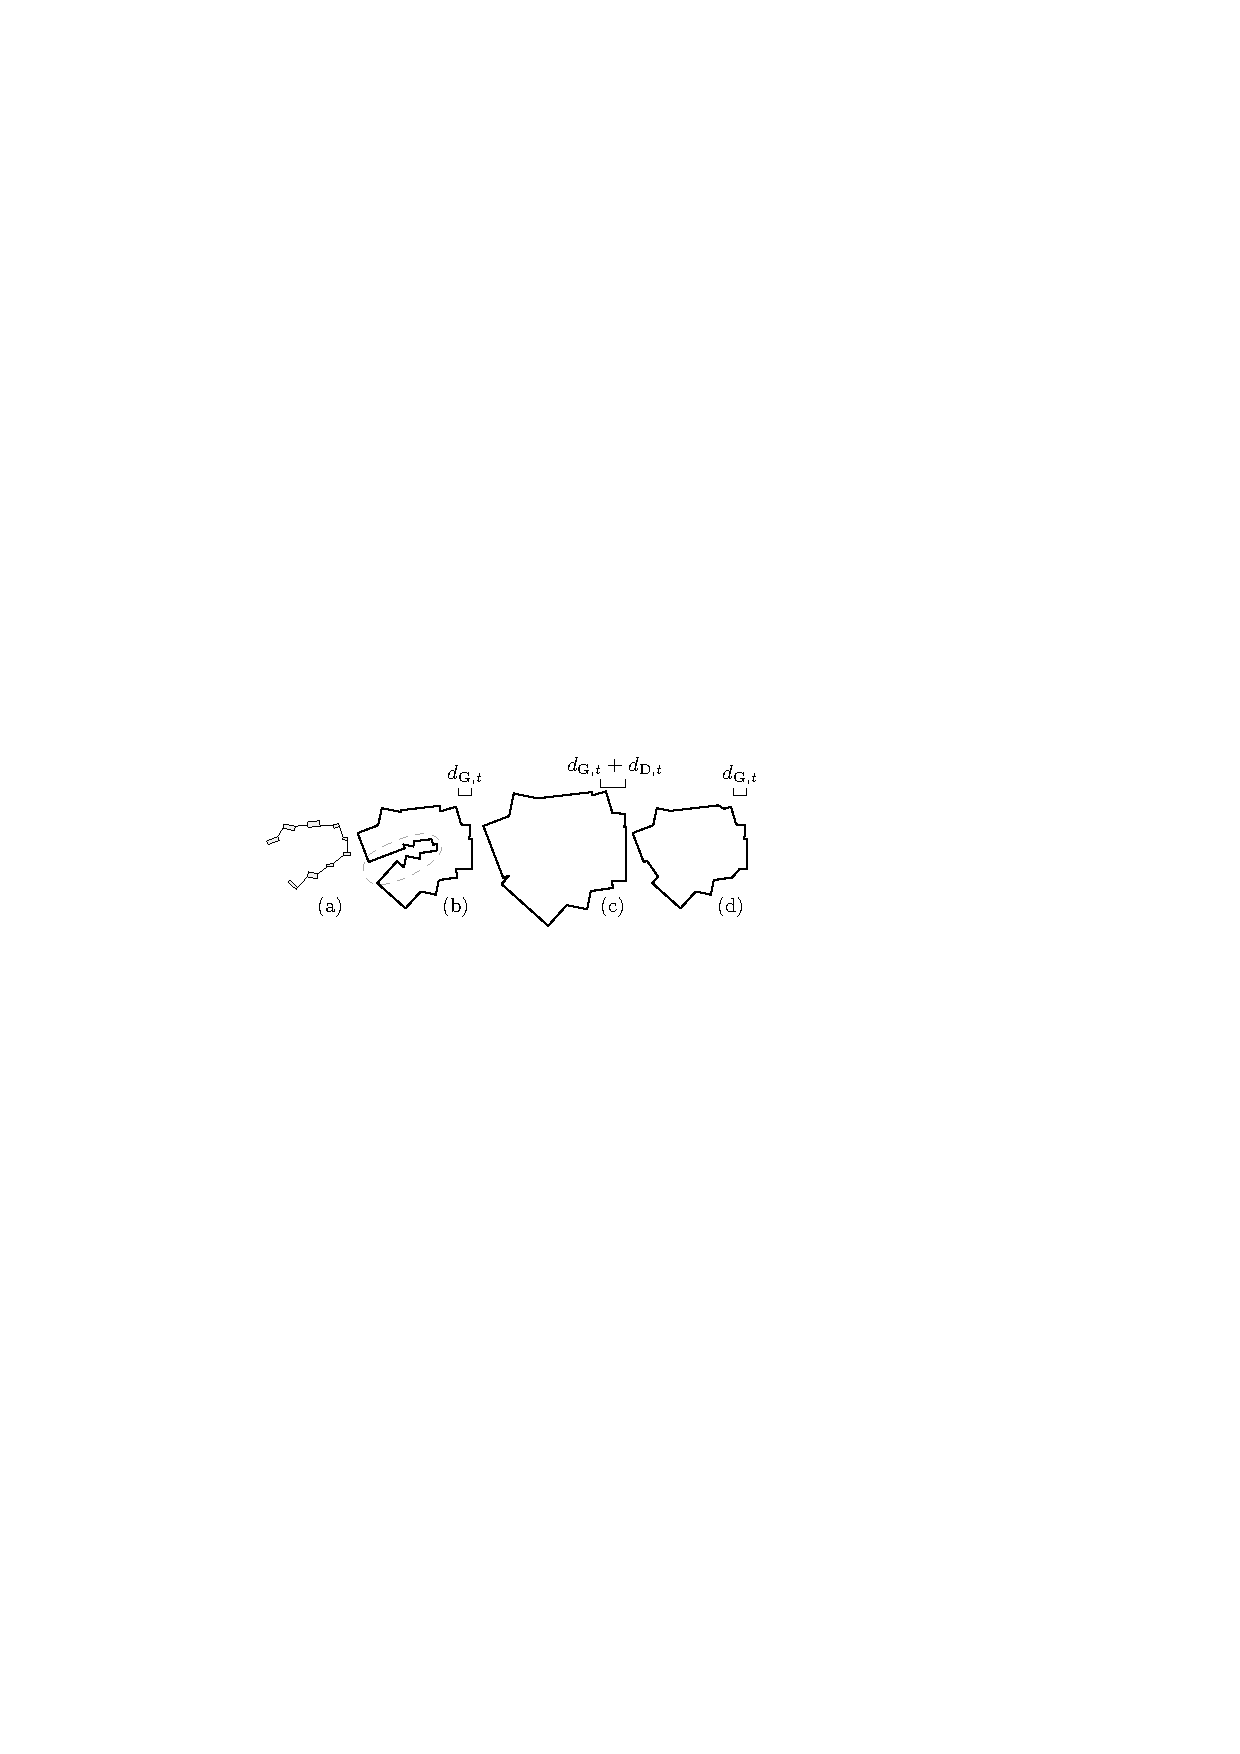
\includegraphics[draft=false]{RemoveBay}
%	\caption{Group buildings iteratively.
%		(a) Original buildings.
%		(b) Dilate each original building with distance 
%		$\dtrm{G}+\dtrm{D}$.		
%		(c) Erode the dilated polygons with distance $\dtrm{D}$.
%		(d) Dilate the eroded polygons with distance $\dtrm{C}$. 
%		If two polygons in (d) intersect, 
%		the original buildings will be put in the same group 
%		because they will become too close at time $t$.
%		There are two groups according to (d).
%		One consists of the single middle building and 
%		the surrounding $9$ buildings comprise the other group.
%		(e) The result of growing and merging at time $t$ 
%		if we use $\dtrm{D}=0$.
%		The process of (f), (g), and (h) is similar to 
%		that of (b), (c), and (d).		
%		The difference is that 
%		instead of applying the operators to each single building, 
%		we do that for the buildings in the same group.
%		In (f), we manage to remove the bay in (e) by additionally dilating 
%		with distance $\dtrm{D}$.
%		There is only one group left according to (h).
%		We iteratively group buildings in this way until the number of groups 
%		does not decrease.
%	}
%	%in this example, we used _dblTotalGrow *= 5;
%	\label{fig:RemoveBay}
%\end{figure*}




%
%
%\subsection{Generating the goal shapes of buildings}
%\label{sec:Goal}
%To generate the goal shapes of buildings, we set time $t=1$.
%We aggregate original buildings (see \sect\ref{sec:Aggregate}).
%Then we grow (see \sect\ref{sec:Grow}) 
%and simplify 
%(see \sects\ref{sec:DilationErosion} and~\ref{sec:ImaiIri}) the grown 
%buildings.
%See for example \fig\ref{fig:GrowAndBridge}, 
%the building at time $t=1$ is the goal shape of the three original buildings.
%
%


\subsection{Generating buildings on intermediate-scale maps}
\label{sec:Unite}

Both the erosion and line simplification may result in shrinking a 
building.
\fig\ref{fig:Shrink_Erosion} and \fig\ref{fig:Shrink_Simplification} show such 
examples respectively.
To avoid these kinds of shrinking,
for a building, we merge its shape at time $t$ 
and its shape at the immediately previous step (before $t$). 
For example, we generate a sequence of $10$ maps,
which means $t \in \{0.1, 0.2, \dots, 1\}$.
\fig\ref{fig:Shrink_Erosion}c shows the result at $t=0.6$.
In \fig\ref{fig:Shrink_Erosion}g, 
the dark-gray part included in the result at $t=0.6$,
but not in the result at $t=0.7$.
In other words, the result at $t=0.7$ shrinks at the dark-gray part.
To prevent the shrinking at $t=0.7$, we merge the result at $t=0.7$ with the 
result of the immediate previous step, i.e., $t=0.6$.
The merged result is shown in \fig\ref{fig:Shrink_Uniting}a.
Similarly, \fig\ref{fig:Shrink_Uniting}b shows the merged result of buildings 
in \fig\ref{fig:Shrink_Simplification}c and~h.

Added to this shrinking problem, a building aggregate on an intermediate map 
should never exceed
the goal shape of the aggregated building. 
Otherwise, the building will need to be shrunk to ensure continuity with the 
goal built-up polygon.
To guarantee this consistency, 
we clip the building using the goal shape 
and remove the outside parts.

\begin{figure}[tb]
	\centering
	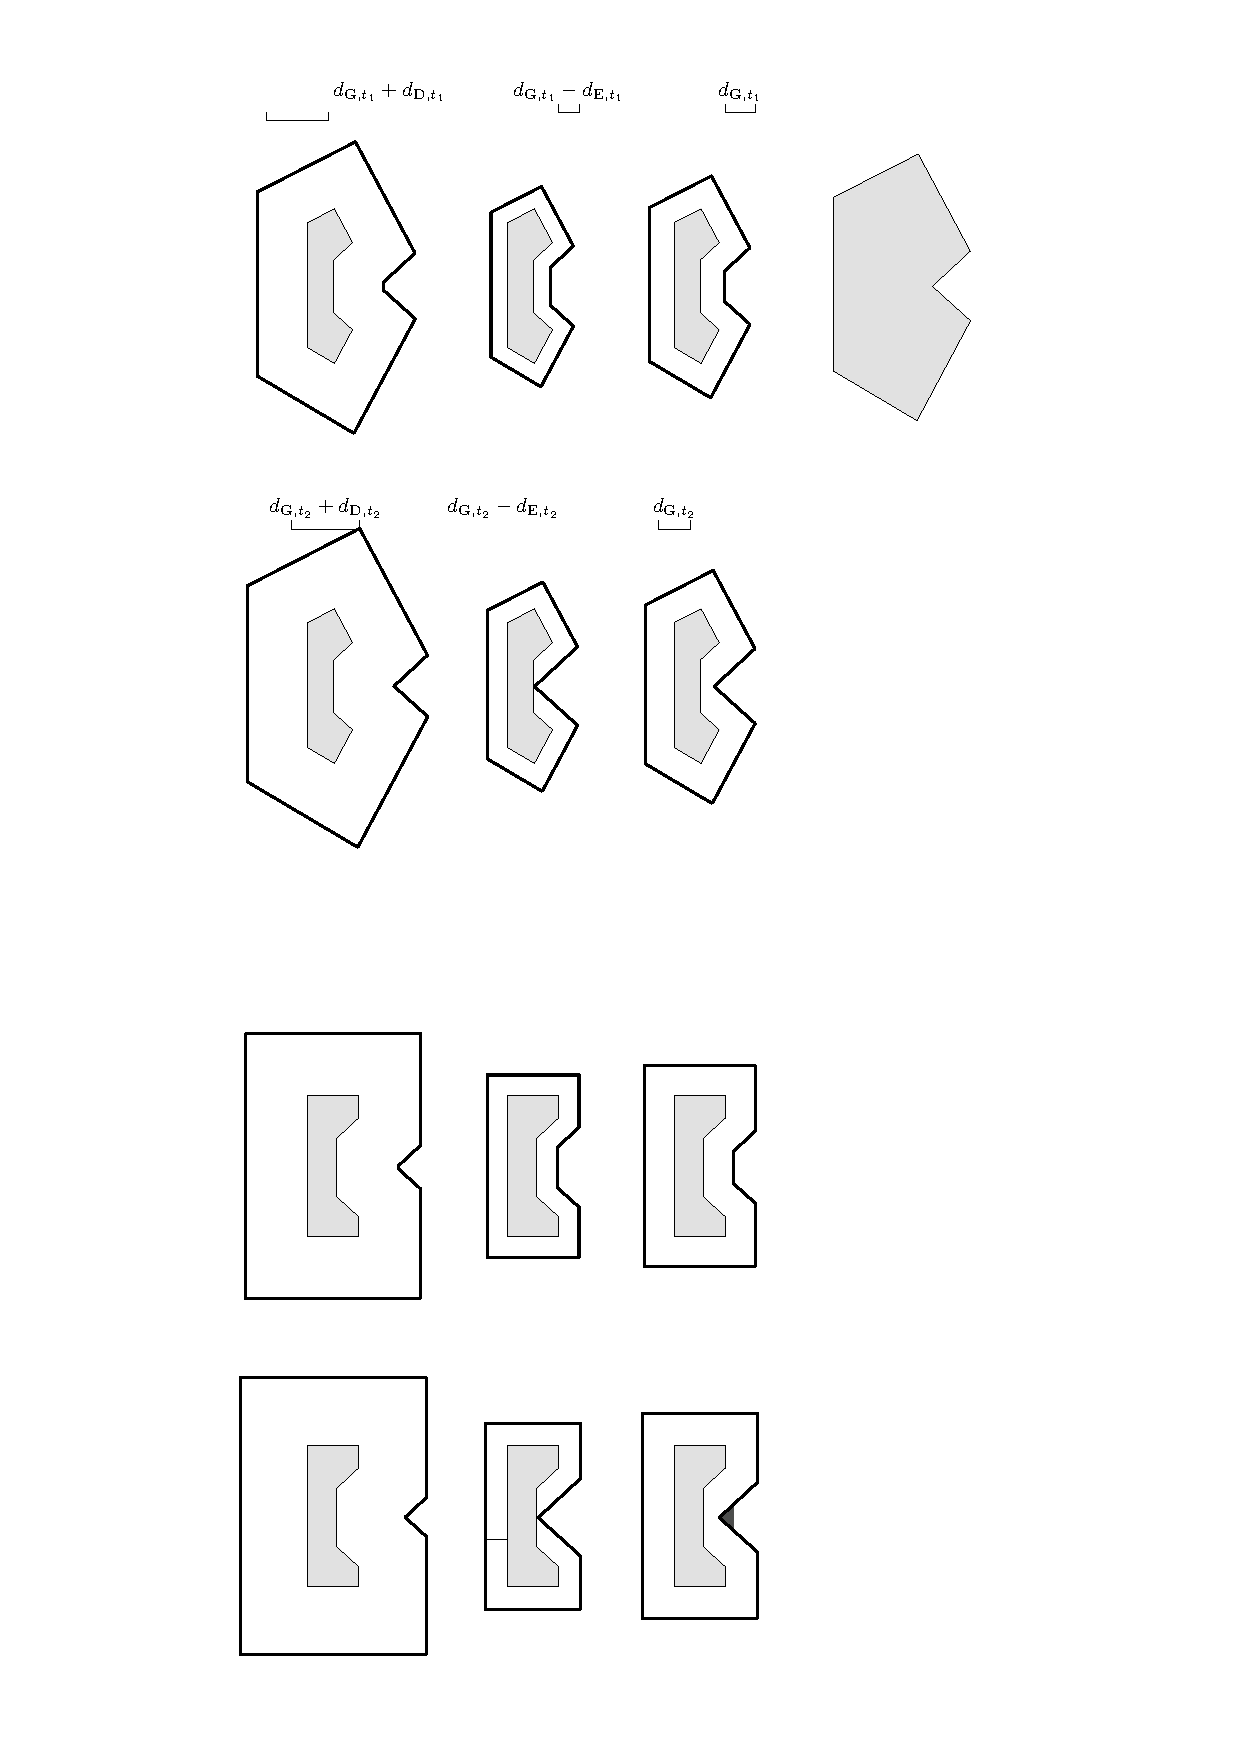
\includegraphics[]{Shrink_Erosion}
	\caption{A building shrinks because of dilation and erosion, 
		where $t_1=0.6$, $t_2=0.7$, and $t_3=1$.
		The gray polygons represent the original building.
		(a) Growing and Dilating the building with distances $\dtrm[1]{G}$ and 
		$\dtrm[1]{D}$, respectively;
		(b) Eroding the polygon in~(a) with $\dtrm[1]{D} + \dtrm[1]{E}$;
		(c) Dilating the polygon in~(b) with $\dtrm[1]{E}$.
		(d) The goal shape.
		The process of (e), (f), and~(g) is the same as the process of (a), 
		(b), and~(c).
		The darker gray piece in (g) shows 
		the part which is included in the polygon of~(c), 
		but not in the polygon of~(g).
	}
	\label{fig:Shrink_Erosion}
\end{figure}

\begin{figure}[tb]
	\centering
	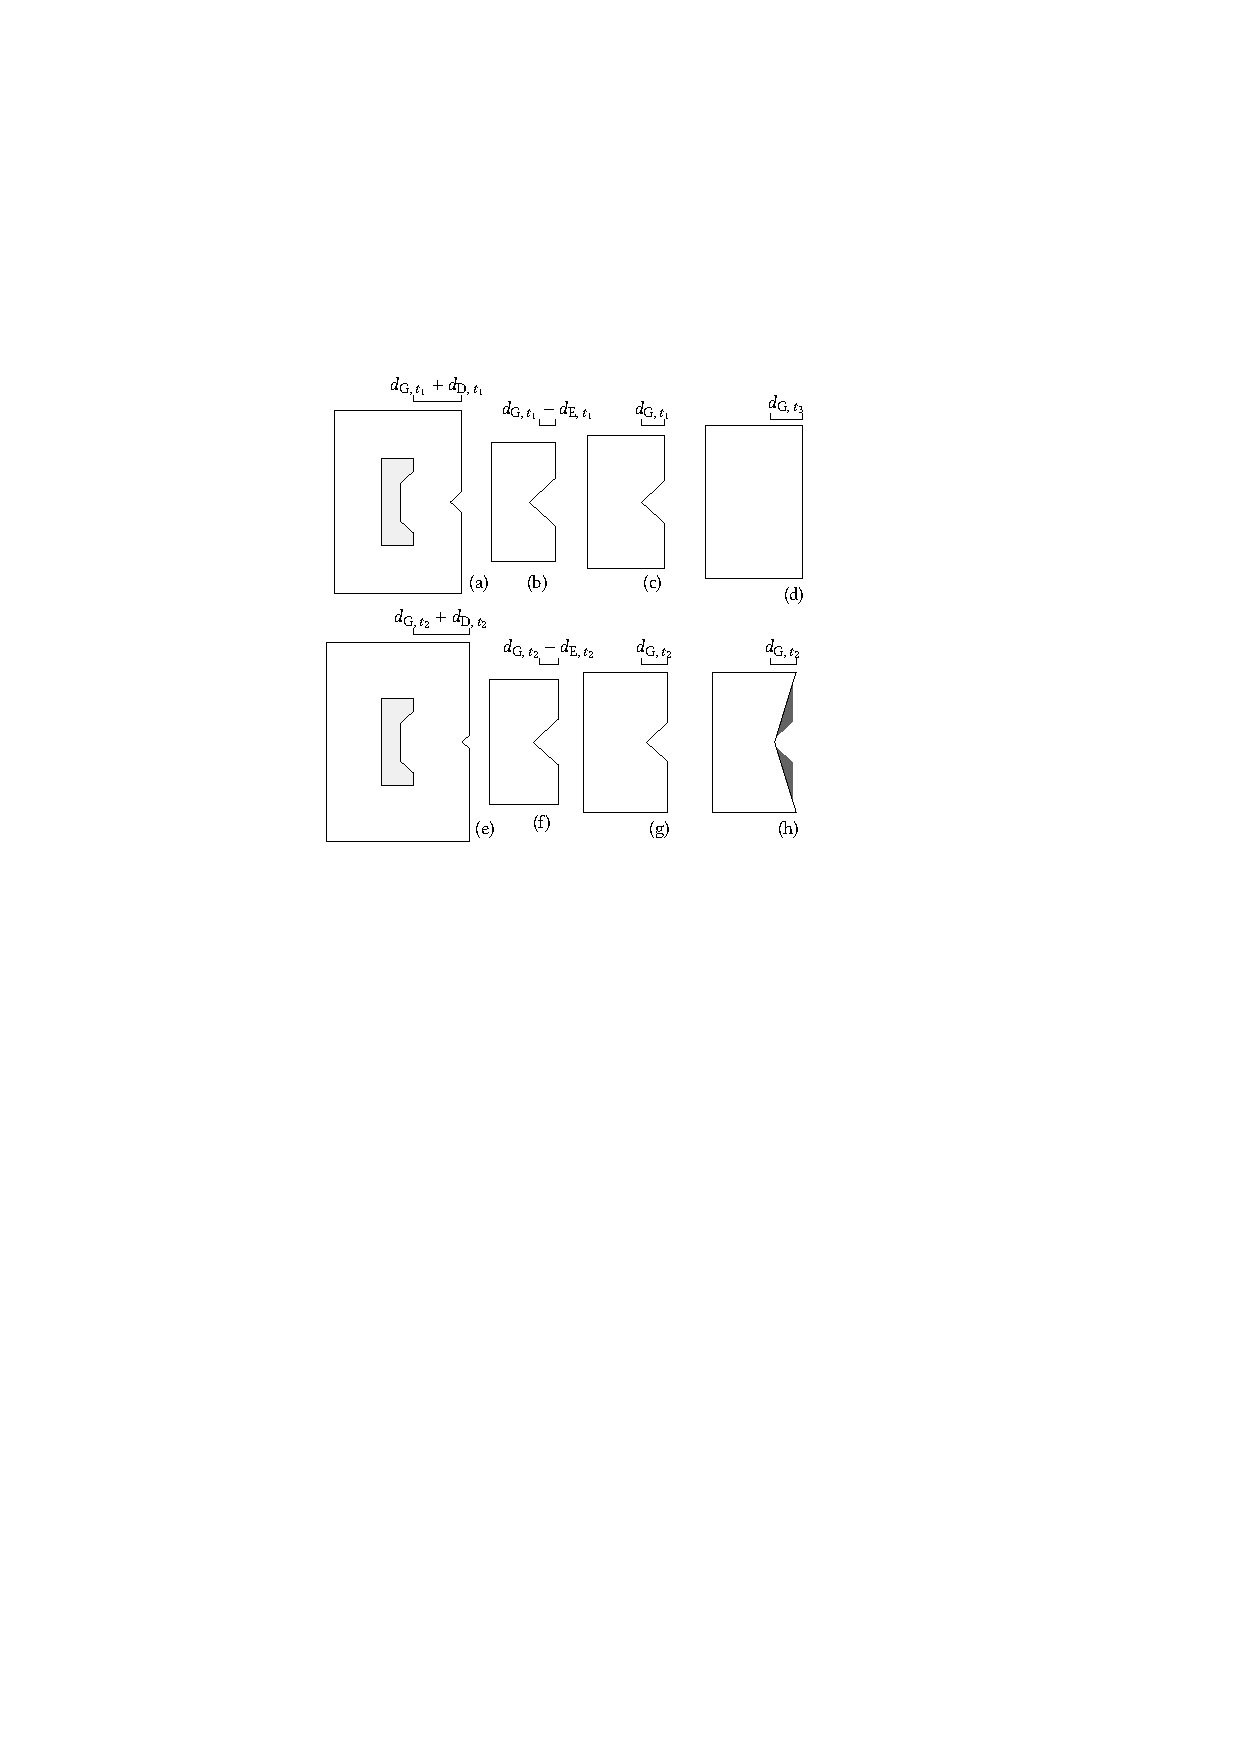
\includegraphics[]{Shrink_Simplification}
	\caption{A building shrinks because of line simplification, 
		where $t_1=0.7$, $t_2=0.8$, and $t_3=1$.
		The gray polygons represent the original building.
		The process of (a), (b), and~(c), and 
		the process of (e), (f), and~(g) are the same as 
		the processes in \fig\ref{fig:Shrink_Erosion}.
		(d) The goal shape.
		(h) Simplifying the polygon in~(g) using the Imai--Iri algorithm.
		Note that $d_{l,t_1}<d_{l,t_2}$ (see \eq\ref{eq:d_lt}),
		which is why the Imai--Iri algorithm does not 
		remove any vertex of the polygon in~(c),
		but removes two vertices of the polygon in~(g).
		The darker gray pieces in~(h) show 
		the parts which are included in the polygon of~(c), 
		but not in the polygon of~(h).
	}
	\label{fig:Shrink_Simplification}
\end{figure}

\begin{figure}[tb]
	\centering
	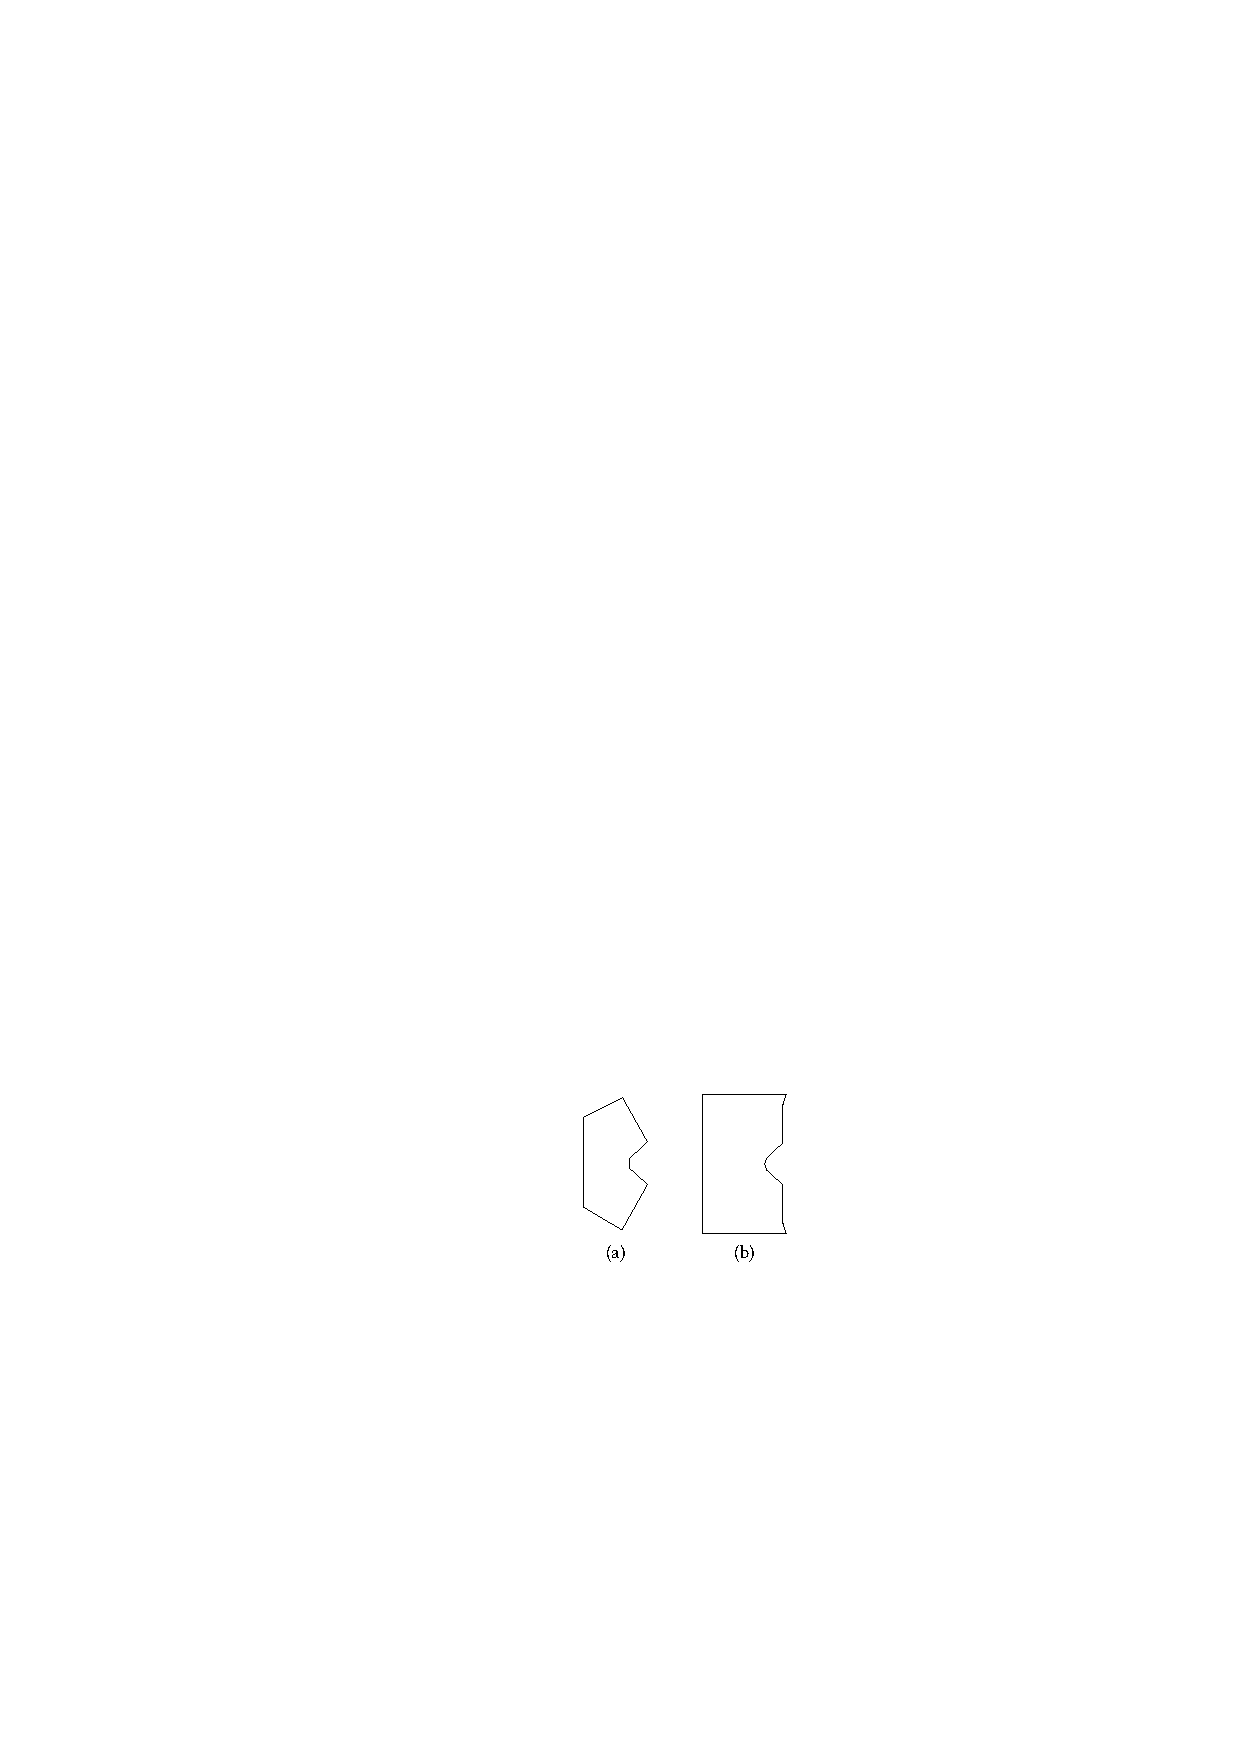
\includegraphics[]{Shrink_Uniting}
	\caption{Merging a polygon with the polygon at the immediately previous 
		step.
		(a) Merging the polygons of \fig\ref{fig:Shrink_Erosion}c and 
		\fig\ref{fig:Shrink_Erosion}g;
		(b) Merging the polygons of \fig\ref{fig:Shrink_Simplification}c and 
		\fig\ref{fig:Shrink_Simplification}h;
	}
	\label{fig:Shrink_Uniting}
\end{figure}




\subsection{Eliminating small buildings}
\label{sec:Eliminate}
Following the previous steps of continuous generalization may result in the 
creation of small isolated building aggregates that do not belong to the goal 
map polygon because of their isolation.
That is why we eliminate a building aggregate if the area of this building is 
smaller than a 
threshold.
Following \citet{Stoter2009} and \citet{Chaudhry2008}, 
we set this threshold as $a=0.16\,\mathrm{mm}^2$ on map.
The real threshold at time $t$ is
\[
a_t=a\cdot M_t^2.
\]
For a group of buildings that will be aggregated into one built-up area at time 
$t=1$, we consider the area sum of all the buildings at time $t$, 
instead of considering each building individually.



%\subsection{Running time analysis}
%Although a version with a 
%lower running time exists \citep[see][]{Chan1992}, we implemented the basic 
%version.


\section{Case Study}
\label{sec:CaseStudy}
We have implemented our method based on
C\# (Microsoft Visual Studio 2015) and ArcObjects SDK 10.4.1.
The offsetting function and clipping function are from library \textsc{Clipper} 
of \citet{Johnson2014}.
The offsetting function realizes 
our operations of buffering, dilating, eroding, and merging.
An evaluation of \textsc{Clipper} can be found in \citet{Palfrader2015}.
We ran our case study under 64-bit 
Windows 7 on a 3.3 GHz dual core CPU with 8 GB RAM.
We measured processing time by the built-in C\# class 
\emph{Stopwatch}.
\fig\ref{fig:Data} shows our testing data, 
which is from the French Mapping Agency (IGN).
The data represents the buildings of four towns (communes in French), 
i.e., Aussevielle, Denguin,  Poey-de-Lescar, and Siros, 
in the Pyr\'en\'ees-Atlantiques department, south-western France.

We set our goal scale at $1:50{,}000$ and $d_\mathrm{G}=25\,\mathrm{m}$
so that we can compare our result with the exiting data.
Also, this setting makes \eq\ref{eq:S_g} hold, 
where $M_\mathrm{g}=50{,}000$, $d_\mathrm{G}=25\,\mathrm{m}$, 
and $l=0.3\,\mathrm{mm}$.
In \eq\ref{eq:d_Dtmin}, the first part is always smaller than the second part 
according to our settings.
As a result $\dtrm{D}=t\cdot 35\,\mathrm{m}$, 
where $\dtrm{E}=t\cdot 7.5\,\mathrm{m}$ 
according to \eq\ref{eq:d_Et} and $\alpha=1.5$.

Our program took $93.6\,\mathrm{s}$ 
to compute the goal shapes of the built-up areas.
\fig\ref{fig:GoalShape} shows the bridged buildings and the goal shapes.
In \fig\ref{fig:GoalShape}b,
the $56$ built-up areas have $2{,}095$ edges before line simplification.
Using the Imai--Iri algorithm, we have $1{,}102$ edges left.
In comparison, there are $1{,}597$ edges left if we simplify using
the Douglas--Peucker algorithm.


\begin{figure}[tb]
	\centering
	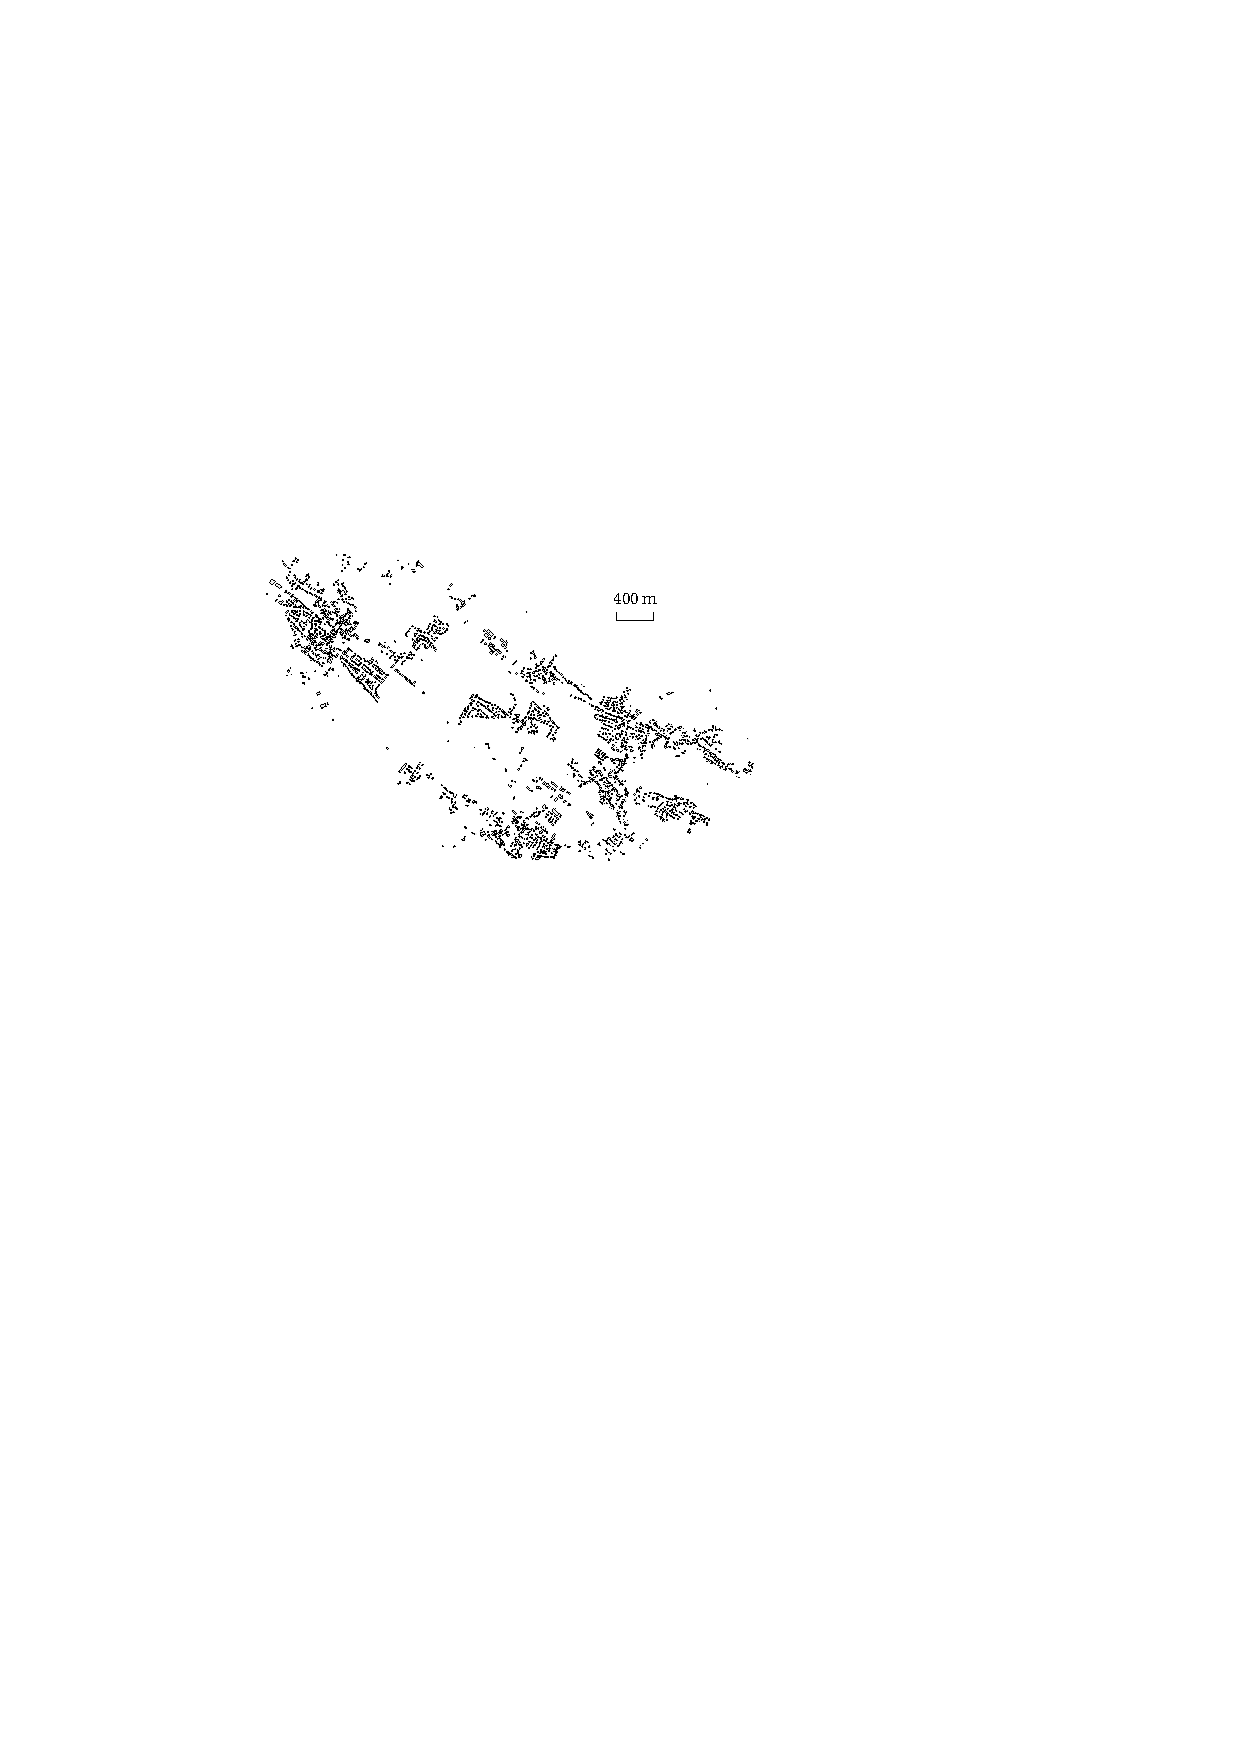
\includegraphics{Data}
	\caption{Data.
		There are $2{,}590$ buildings, 
		which have $19{,}255$ edges in total.}
	\label{fig:Data}
\end{figure}


\begin{figure*}[tb]
	\centering
	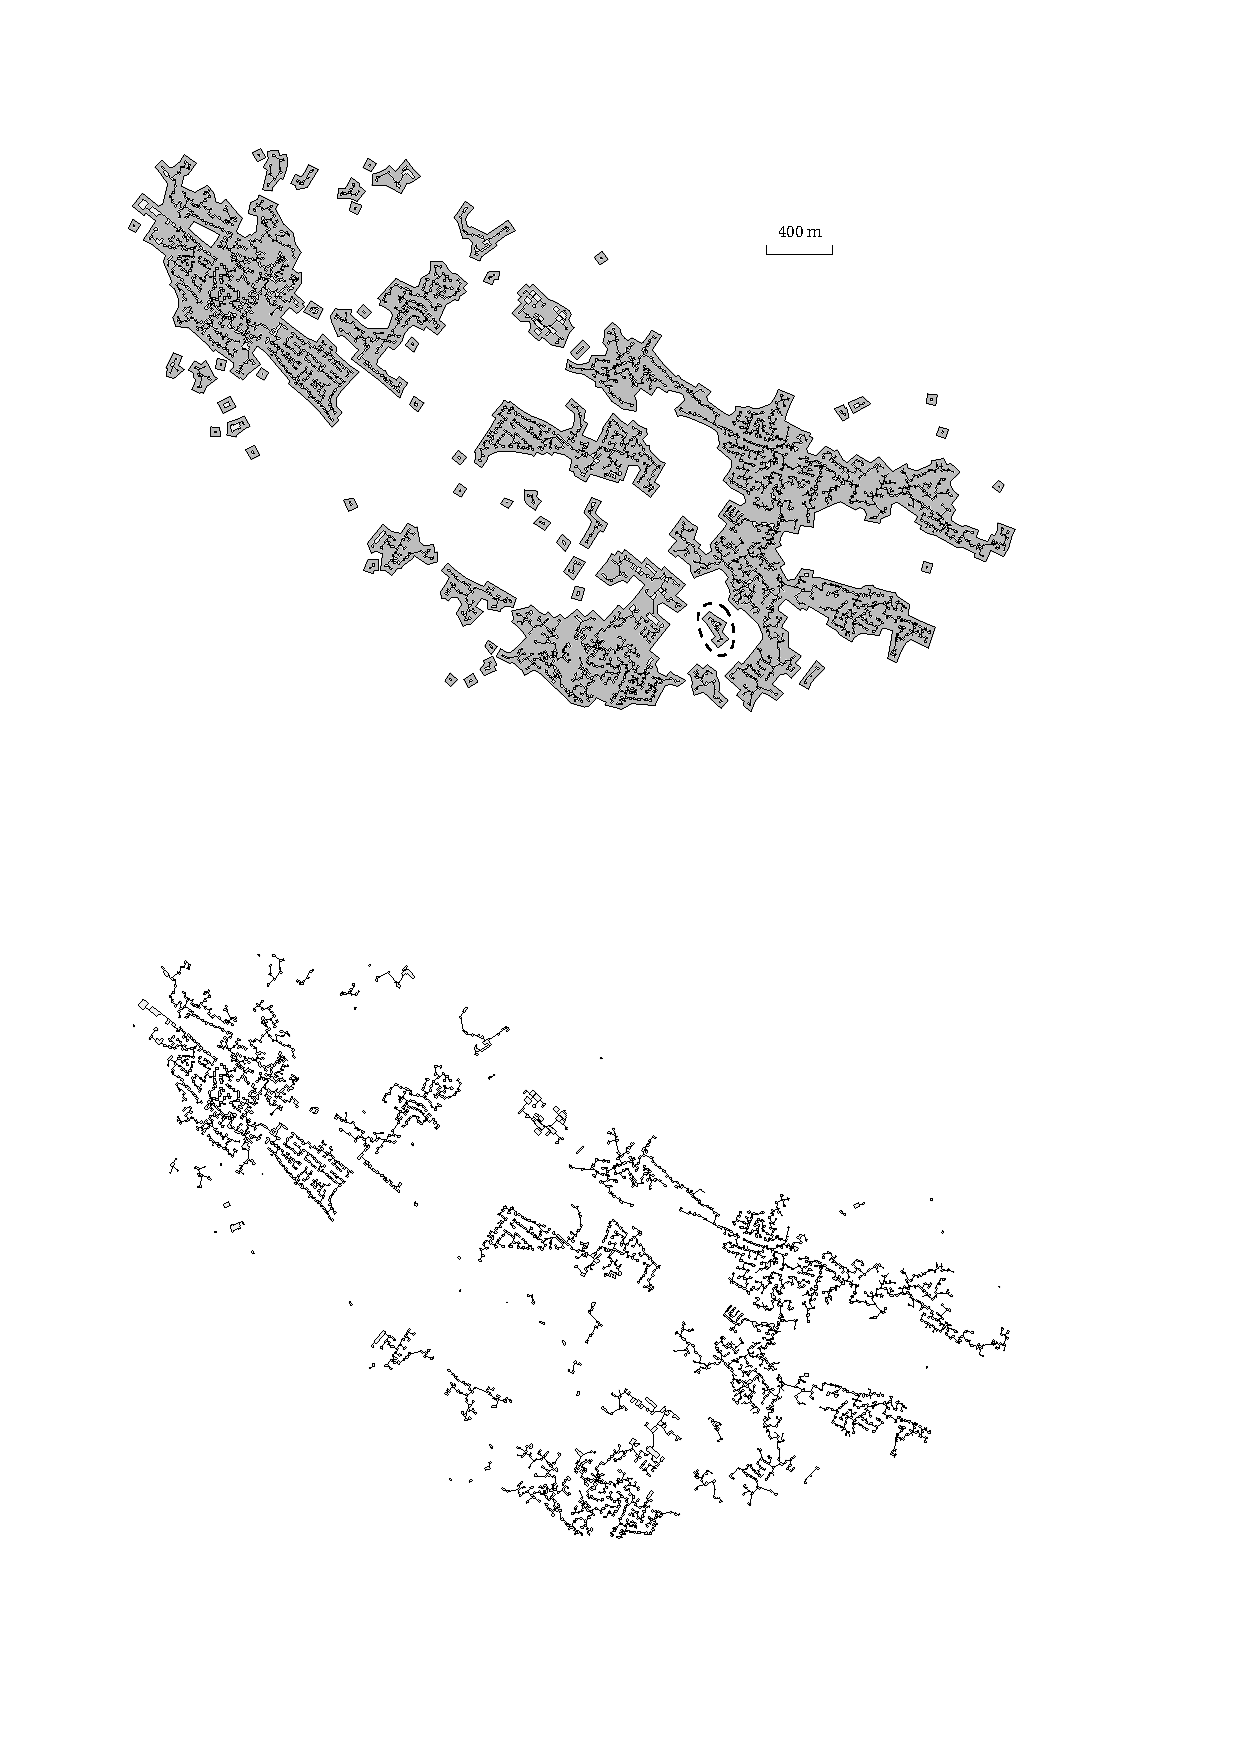
\includegraphics{GoalShape}
	\caption{Bridged original buildings 
		and goal shapes of the built-up areas (without removing small holes), 
		at scale $1:50{,}000$.
		There are $56$ built-up areas, which have $1{,}102$ edges in total.
	}
	\label{fig:GoalShape}
\end{figure*}

\begin{figure*}[tb]
	\centering
	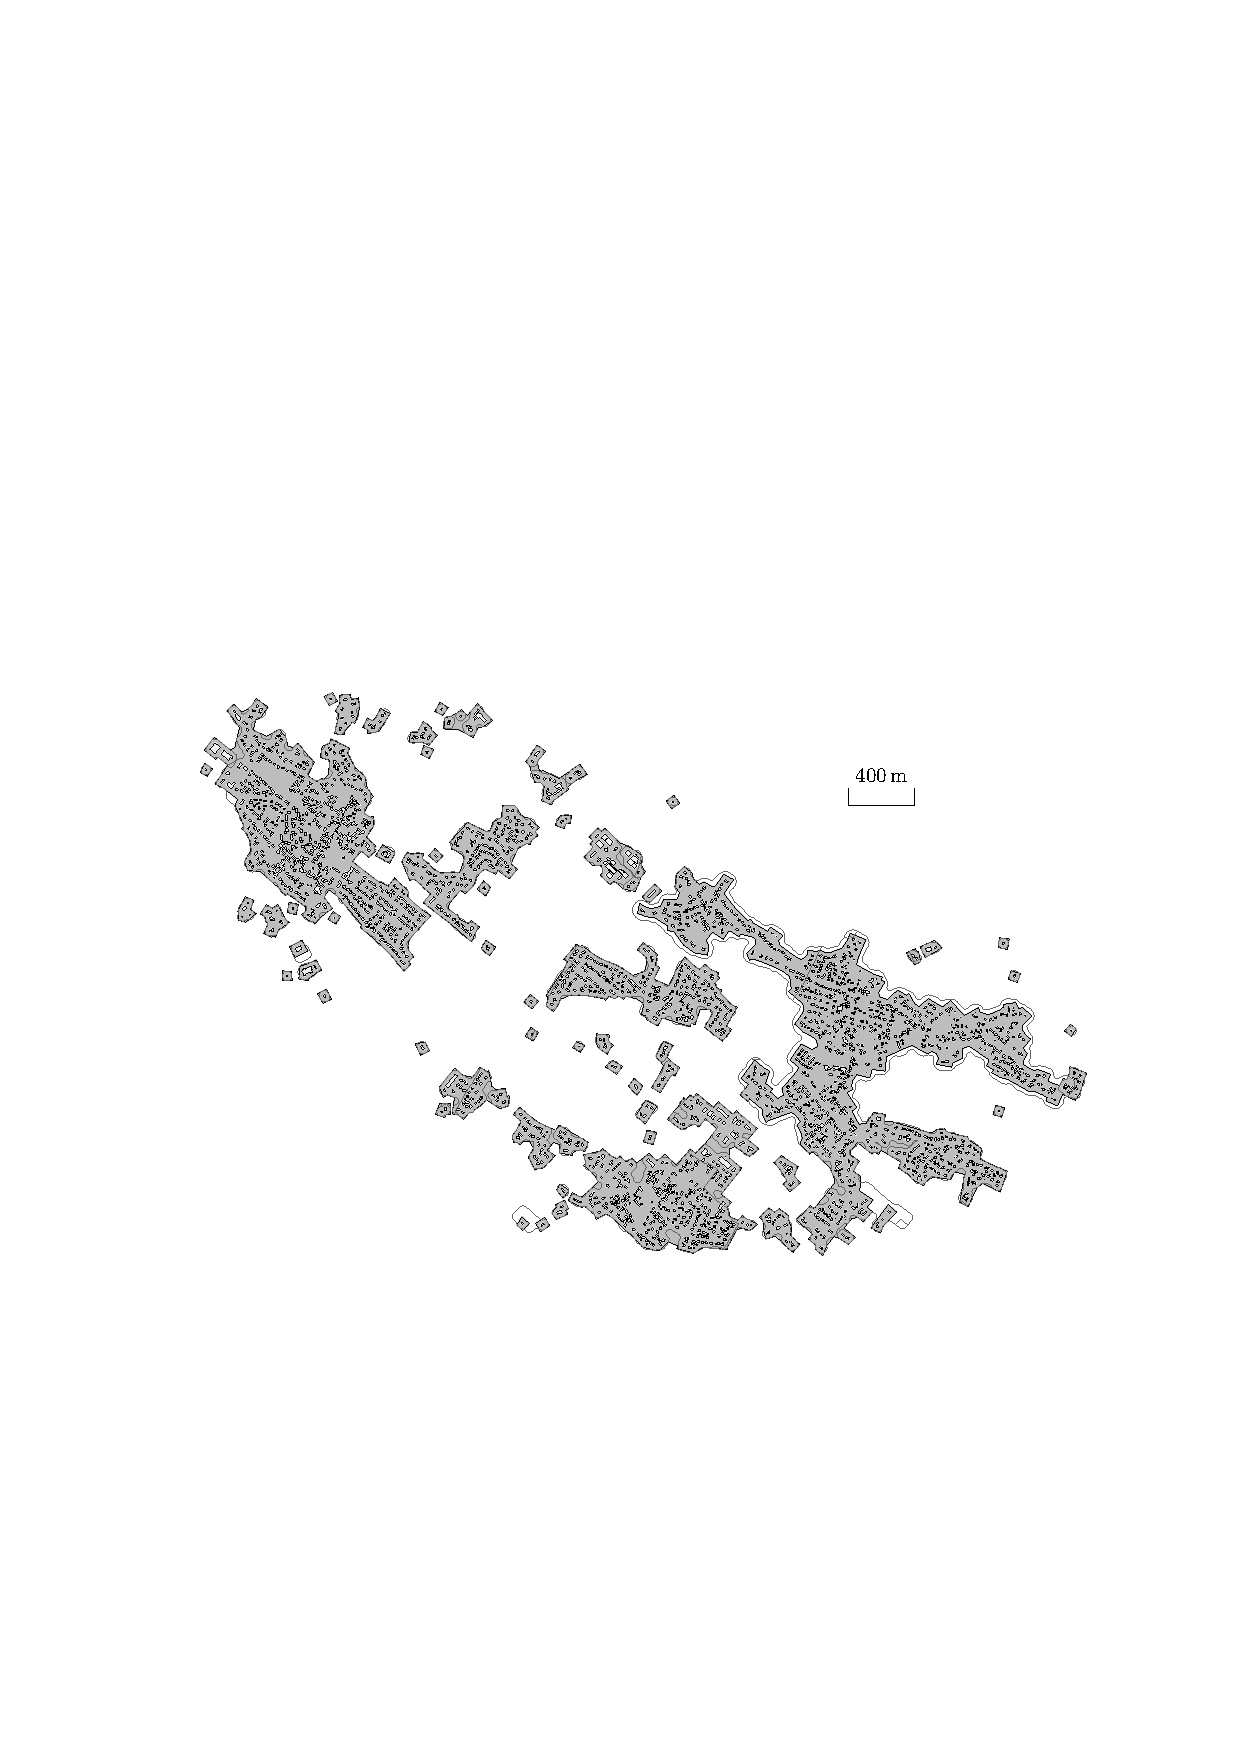
\includegraphics{ExperimentalComparison}
	\caption{.
	}
	\label{fig:ExperimentalComparison}
\end{figure*}


The area on start map is $some number\,\text{mm}^2$.
Our area on map is $some number\,\text{mm}^2$.
According to \eq4 of paper \citet{Topfer1966}, 
the area on map should be $some number\,\text{mm}^2$

%Although a version with a 
%lower running time exists \citep[see][]{Chan1992}, we implemented the basic 
%version

\section{Conclusion}
\label{sec:Conclusion}


Our intermediate results may violate more cartographic rules, but we try to 
make the results at goal scales violate as few rules as possible.


Eventually, our result is a set of settlement boundaries. An interesting 
problem is to compare our method with \citet{Chaudhry2008}.

We used radical law. We may also consider the fractal nature of maps proposed 
by \citet{Jiang2015}.

We did not include streets. We can either put them above the settlement 
boundaries on map, or use them as restriction for building growing.

Show some results obtained by ArcGIS.
Show the data at $1:50{,}000$.

A special kind of Voronoi diagram considering miter offset. A buildings is 
allowed to grow inside its own zone.

\todo[inline]{consider multi bridges; 
	consider transparency of bridges in stead of enlarging}